\documentclass[12pt, oneside]{report}
\usepackage{IEEEtrantools}

\usepackage[margin=2.5cm]{geometry}
\linespread{1.5}
\usepackage{hyperref}
\usepackage{mathptmx}
\usepackage{xcolor}
\usepackage{hyperref}
%\usepackage[style=authoryear, defernumbers=true, backend=biber,dashed=false, maxnames=999,maxcitenames=2,giveninits=true,urldate=long,uniquename=false,uniquelist=false]{biblatex}
\usepackage[style=ieee]{biblatex}




\addbibresource{References.bib}
%\addbibresource{biblio.bib}

%% pretty captions
\usepackage{caption}
\usepackage{subcaption}
%%% allows you to create Rules, Definitions, Lemmas, Theorems etc.
\usepackage{amsthm}
\usepackage{amsmath}
\usepackage{amsfonts}
\usepackage[]{algorithm2e}

\newtheorem{theorem}{Theorem}
\newtheorem{definition}{Definition}
\newtheorem{lemma}{Lemma}
\newtheorem{Rule}{Rule}
\numberwithin{definition}{chapter}
\numberwithin{theorem}{chapter}  
\numberwithin{lemma}{chapter}  
\numberwithin{Rule}{chapter}  
\numberwithin{equation}{chapter} 
\newcommand\tab[1][1cm]{\hspace*{#1}}

 \usepackage[super]{nth} 
 
\usepackage{graphicx}
\usepackage{wrapfig}
\usepackage{placeins}
\usepackage{pdfpages}
\usepackage{attachfile2}

\usepackage[utf8]{inputenc}
\usepackage[T1]{fontenc}
\usepackage{csquotes}

\usepackage{fancyhdr}
%\pagestyle{fancy}
\renewcommand{\headrulewidth}{0.4pt}
%\renewcommand{\footrulewidth}{0.4pt}
\fancyhead{}
\fancyhead[L]{SHORTENED TITLE} %%% CHANGE AS APPROPRIATE (you may need to use a shortened form of the title)
\fancyhead[R]{Student ID: .......} %%% CHANGE AS APPROPRIATE
\fancyfoot{}
\fancyfoot[C]{\thepage}

\usepackage{titlesec}
\titlespacing{\chapter}{0pt}{*4}{*2.5}

\usepackage{indentfirst} % 首行缩进命令
\usepackage{amssymb} % 更多符号


\newcommand{\comment}[1]{} % \comment{} 花括号中的内容会被视为注释,也就实现了块注释,vscode的场合,ctrl+/也可以的


\titleformat{\chapter}{\normalfont\huge\bf}{\thechapter}{20pt}{\huge\bf}
%% prevents Chapter 1 (then new line and Introduction) - turns into 1. Introduction


%% Call your references "References" rather than Bibliography, then also allow for a separate Bibliography if needed.

\DeclareSourcemap{
  \maps[datatype=bibtex]{
    \map{
      \perdatasource{references.bib}
      \step[fieldset=keywords, fieldvalue={, primary}, append]
    }
    \map{
      \perdatasource{biblio.bib}
      \step[fieldset=keywords, fieldvalue={, secondary}, append]
    }
  }
}
%%%%%%%%%%%%%%%%%%%%%%%%%%%%%%%%
%  Don't make any changes here
%  This defines formatting style
%%%%%%%%%%%%%%%%%%%%%%%%%%%%%%%%

\DeclareNameAlias{sortname}{last-first}
\DeclareFieldFormat{edition}{%
  \ifinteger{#1}
    {\ifnumequal{#1}{1}%
     {}%
     {\mkbibordedition{#1}~\bibstring{edition}}%
    }
    {#1\isdot}}

\DeclareFieldFormat[article,inbook,incollection]{title}{#1\isdot}
\DeclareFieldFormat[article,inbook,incollection]{citetitle}{#1\isdot}

\newrobustcmd{\MakeTitleCase}[1]{%
  \ifboolexpr{test {\ifentrytype{article}} or test {\ifentrytype{inbook}} or test {\ifentrytype{incollection}}}
    {#1}
    {\MakeSentenceCase{#1}}}

\DeclareFieldFormat{urldate}{\bibsentence\mkbibbrackets{\bibstring{urlseen}\space#1}}
\DeclareFieldFormat{url}{\bibstring{urlfrom}\addcolon\space\url{#1}}

\renewbibmacro*{journal}{%
  \iffieldundef{journaltitle}
    {}
    {\printtext[journaltitle]{%
       \printfield[titlecase]{journaltitle}%
       \setunit{\subtitlepunct}%
       \printfield[titlecase]{journalsubtitle}}
       \ifboolexpr{
         not test {\iffieldundef{url}}
         or
         not test {\iffieldundef{urldate}}
         or
         not test {\iffieldundef{doi}}
         or
         not test {\iffieldundef{eprint}}
       }
         {\nopunct\bibstring[\mkbibbrackets]{online}}%
         {}}}

\renewbibmacro*{journal+issuetitle}{%
  \usebibmacro{journal}%
  \setunit*{\addspace}%
  \iffieldundef{series}
    {}
    {\newunit
     \printfield{series}%
     \setunit{\addspace}}%
  \newunit
  \usebibmacro{volume+number+eid}%
  \setunit{\addspace}%
  \usebibmacro{issue+date}%
  \setunit{\addcolon\space}%
  \usebibmacro{issue}%
  \newunit}

\NewBibliographyString{online}
\DefineBibliographyStrings{english}{%
  urlseen    = {accessed},
  online     = {online},
}
%\addbibresource{example.bib}
\renewcommand*{\nameyeardelim}{\addcomma\addspace}
\renewbibmacro{in:}{%
  \ifentrytype{article}{}{\printtext{\bibstring{in}\intitlepunct}}} % removes "In" preceeding journal title
\setcounter{tocdepth}{1} % allow only sections (not subsections in table of contents)

\begin{document}
\begin{titlepage}
    \begin{center}
        \vspace*{1cm}
        {\huge
        Decentralised Multi-Agent Path Planning based on Self-Organised Time Division Multiple Access}
        \vspace{0.5cm}
        \\
        {\large By}
        \\
        \vspace{0.5cm}
        \textbf{Runze Yuan}
   		\vspace{1.5cm}
        \center{\huge{\textbf{MSc Robotics Dissertation}}}
        \\
        \vspace{0.25cm}
       
\includegraphics[scale=0.6]{logos/bristolcrest_colour.pdf}
        \hspace{5mm}
        
\includegraphics[scale=0.35]{logos/UWE_insignia.png}

        \vspace{10mm}
        {\large Department of Engineering Mathematics\\
        \textsc{University of Bristol}}
        \\
        \&
        \\
        {\large Department of Engineering Design and Mathematics\\
        \textsc{University of the West of England}}\\

        \vspace{0.8cm}
        \begin{minipage}{10cm}
        \center A MSc dissertation submitted to the University of Bristol and the University of the West of England in accordance with the requirements of the degree of \textsc{Master of Science in Robotics} in the Faculty of Engineering.
        \end{minipage}\\
        \vspace{0.8cm}
        \today
        
    \end{center}
    
 

\end{titlepage}
\chapter*{Declaration of own work}

I declare that the work in this MSc dissertation was carried out in accordance with the requirements of  the University's Regulations and Code of Practice for Research Degree Programmes and that it  has not been submitted for any other academic award. Except where indicated by specific  reference in the text, the work is the candidate's own work. Work done in collaboration with, or with the assistance of, others, is indicated as such. Any views expressed in the dissertation are those of the author.


 \begin{flushright}
 
 Name and Date
\end{flushright}

\newpage
\chapter*{Acknowledgement}
% Add here text if you would like to thank somebody, e.g., your family, friends, colleagues, supervisors, etc.

I would like to thank ... 


\chapter*{Abstract}
\textbf{
Abstract should give a short summary of the motivation, the approach and important insights and results.}
%
\vfill
\begin{flushright}
 Number of words in the dissertation: .... words.
\end{flushright}
    
 %% any other "Front matter" should go here before the table of contents - format in a style similar to the file Abstract.tex
\tableofcontents 
\listoftables
\addtocontents{toc}{~\hfill\textbf{Page}\par} % comment this line out if you want to remove "Page"
%%%%%%%%%%%%%%%%%%%%%%%%%%%%%%%%%%%%
\chapter{Introduction}
\label{chap:Introduction}
%%%%%%%%%%%%%%%%%%%%%%%%%%%%%%%%%%%%

\comment{

The introduction should provide:
\begin{itemize}
    \item A clear explanation of the problem that you tackle
    \item Motivation why this is interesting and worth investigating
\end{itemize}

To improve communication, it is also recommended that you concisely state the aims and objectives of your project.  As part of the introduction, these can be generally stated and not require specialist knowledge.  Use the next chapter "Literature Review" to provide specialist knowledge for the reader.
\begin{enumerate}
    \item \textbf{Aims:} The aims of a project are \emph{what you hope to learn}.
        \begin{enumerate}
        \item "To understand why X varies with Y..."
        \item "To evaluate [technology] when exposed to unexpected conditions so that..."
        \item "To increase understanding of ..."
        \item \emph{etc...}
        \end{enumerate}
    \item \textbf{Objectives:} The objectives are \emph{the elements which are necessary to conduct the project}.
        \begin{enumerate}
            \item "To properly design an experiment methodology to mitigate...."
            \item "To construct a robotic system including ... to collect meaningful data."
            \item "A complete analysis of ... must be conducted prior to the full system evaluation in order to..."
            \item \emph{etc...}
        \end{enumerate}
\end{enumerate}

You can then repeat and address these explicitly in your Conclusion when evaluating the success and challenges of your project. 

}

\section{Aims}

Based on the self-organised channel resource allocation principle of the STDMA
(Self-organised Time Division Multiple Access) \cite{STDMA} communication protocol, develop
a method for agents to achieve collision-free moving on a 2D plane, make it self-organised,
decentralised and scalable.

% 注意,这里后面可以用一个itemize将算法所需要达到的性能展开说


\section{Objectives}

% 注:objectives里面后续可以加上为什么要这么做,譬如:为了观察。。。,必须构建一个。。。

\begin{itemize}
    \item  Develop a multi-agent communication scenario with STDMA in ROS2. In this 
    scenario, multiple identical agents will share the same channel and all agents
    have both receiving and transmitting capabilities. The goal is to enable agents to
    autonomously organise/join the communication process after start up. 
    \item On the basis above, a grid world is implemented: a 2D map composed of grids, 
    each grid represent a part of space. Agents could move from one grid to another in the map.
    \item \dots
\end{itemize}

\section{Motivation}

The motivation of this project is to answer a question inspired by \cite{Paper_From_Supervisor}, which is:

\begin{quote}
    \textbf{What will happen if use STDMA for 2D resource sharing?}
\end{quote}

The detailed explanation of the motivation is as follows.

\subsection{Why STDMA?}

\label{sec:Why STDMA?}

\textbf{What is STDMA?} The \textit{Self-organised Time Divided Multi Access} (STDMA)
 is an channel access technique for communication. 
 It is based on a set of policies dictating how agents ought to apply for
  slots in repeating frames. 
  In short, STDMA is a protocol that allows agents to autonomously
   share 1D resources (time) among themselves.

   % 记得加上:详细的解释位于文献综述部分

The reason for using STDMA is its \textbf{characteristics}:

\begin{enumerate}
    \item \textbf{Deterministic}: Agents arrange their data transmission based on a determined timetable.
    \item \textbf{Decentralised}: Agents listen to the channel first, then find free slots in the timetable for themselves to use.
\end{enumerate}

These characteristics could be useful for multiple agents to achieve collision-free (use free slots only),
 self-organised (find slots on its own) resource sharing.

There are also two \textbf{reasons that making this challenging}: 

\begin{enumerate}
    \item \textbf{Purpose difference}: In the original STDMA, an agent only needs to find one unused slot
    in the repeating frame (which is generally of a fixed length chosen manually) and maintain ownership of that slot,
    which means agents don't need to move from one slot to another slot, i.e., don't have destination in the channel allocation timetable. 
    But that's different for 2D space moving, where agents have their destinations and need to move grid by grid to reach their goals.
    % 这里可以补一句话,关于如果直接使用在2D中会导致的可能结果。来具体说明这种用途的不同到底会造成什么结果
    \item \textbf{Complexity difference}: Channel sharing only requires randomly selecting one slot from the known free slots, while space sharing in
     a 2D plane requires the agent to find a path that doesn't collide with other agents, and the possibility space for the path could be enormous
      (map size $\times$ predicting horizon), but the processing time available to the agent is limited
       (must broadcast its presence at regular intervals so that other agents can be aware of its plans and thus avoid collisions).
\end{enumerate}


These characteristics and challenges make this project interesting and worthy of research.


\subsection{Why 2D plane path planning?}

2D plane path planning is a name for better understanding and is not the accurate name for this problem.
This problem is acturally a \textbf{\textit{Multi-Agent Path Finding} (MAPF)} problem \cite{MAPF_Explain1, MAPF_Explain2}.

Here, the term "finding" could be somewhat confusing. 
In fact, he MAPF problem combines both \textbf{collision-free movement} of multiple agents and 
\textbf{path efficiency optimising}.

Overall, the problem of \textit{Multi-Agent Path Finding} (MAPF) concerns \textbf{the movement of multiple agents in a grid world}.

To easily get a better understanding of this problem, please refer to this \href{https://primalgrid.netlify.app/primal}{website}\footnotemark.\footnotetext{https://primalgrid.netlify.app/primal}
The website presents the MAPF problems and their solutions through a simple and engaging animation (estimated time required: 1$\sim$2 min).

% 记得加上:详细描述参看后续Literature review

%\FloatBarrier
\begin{figure}
    \centering
    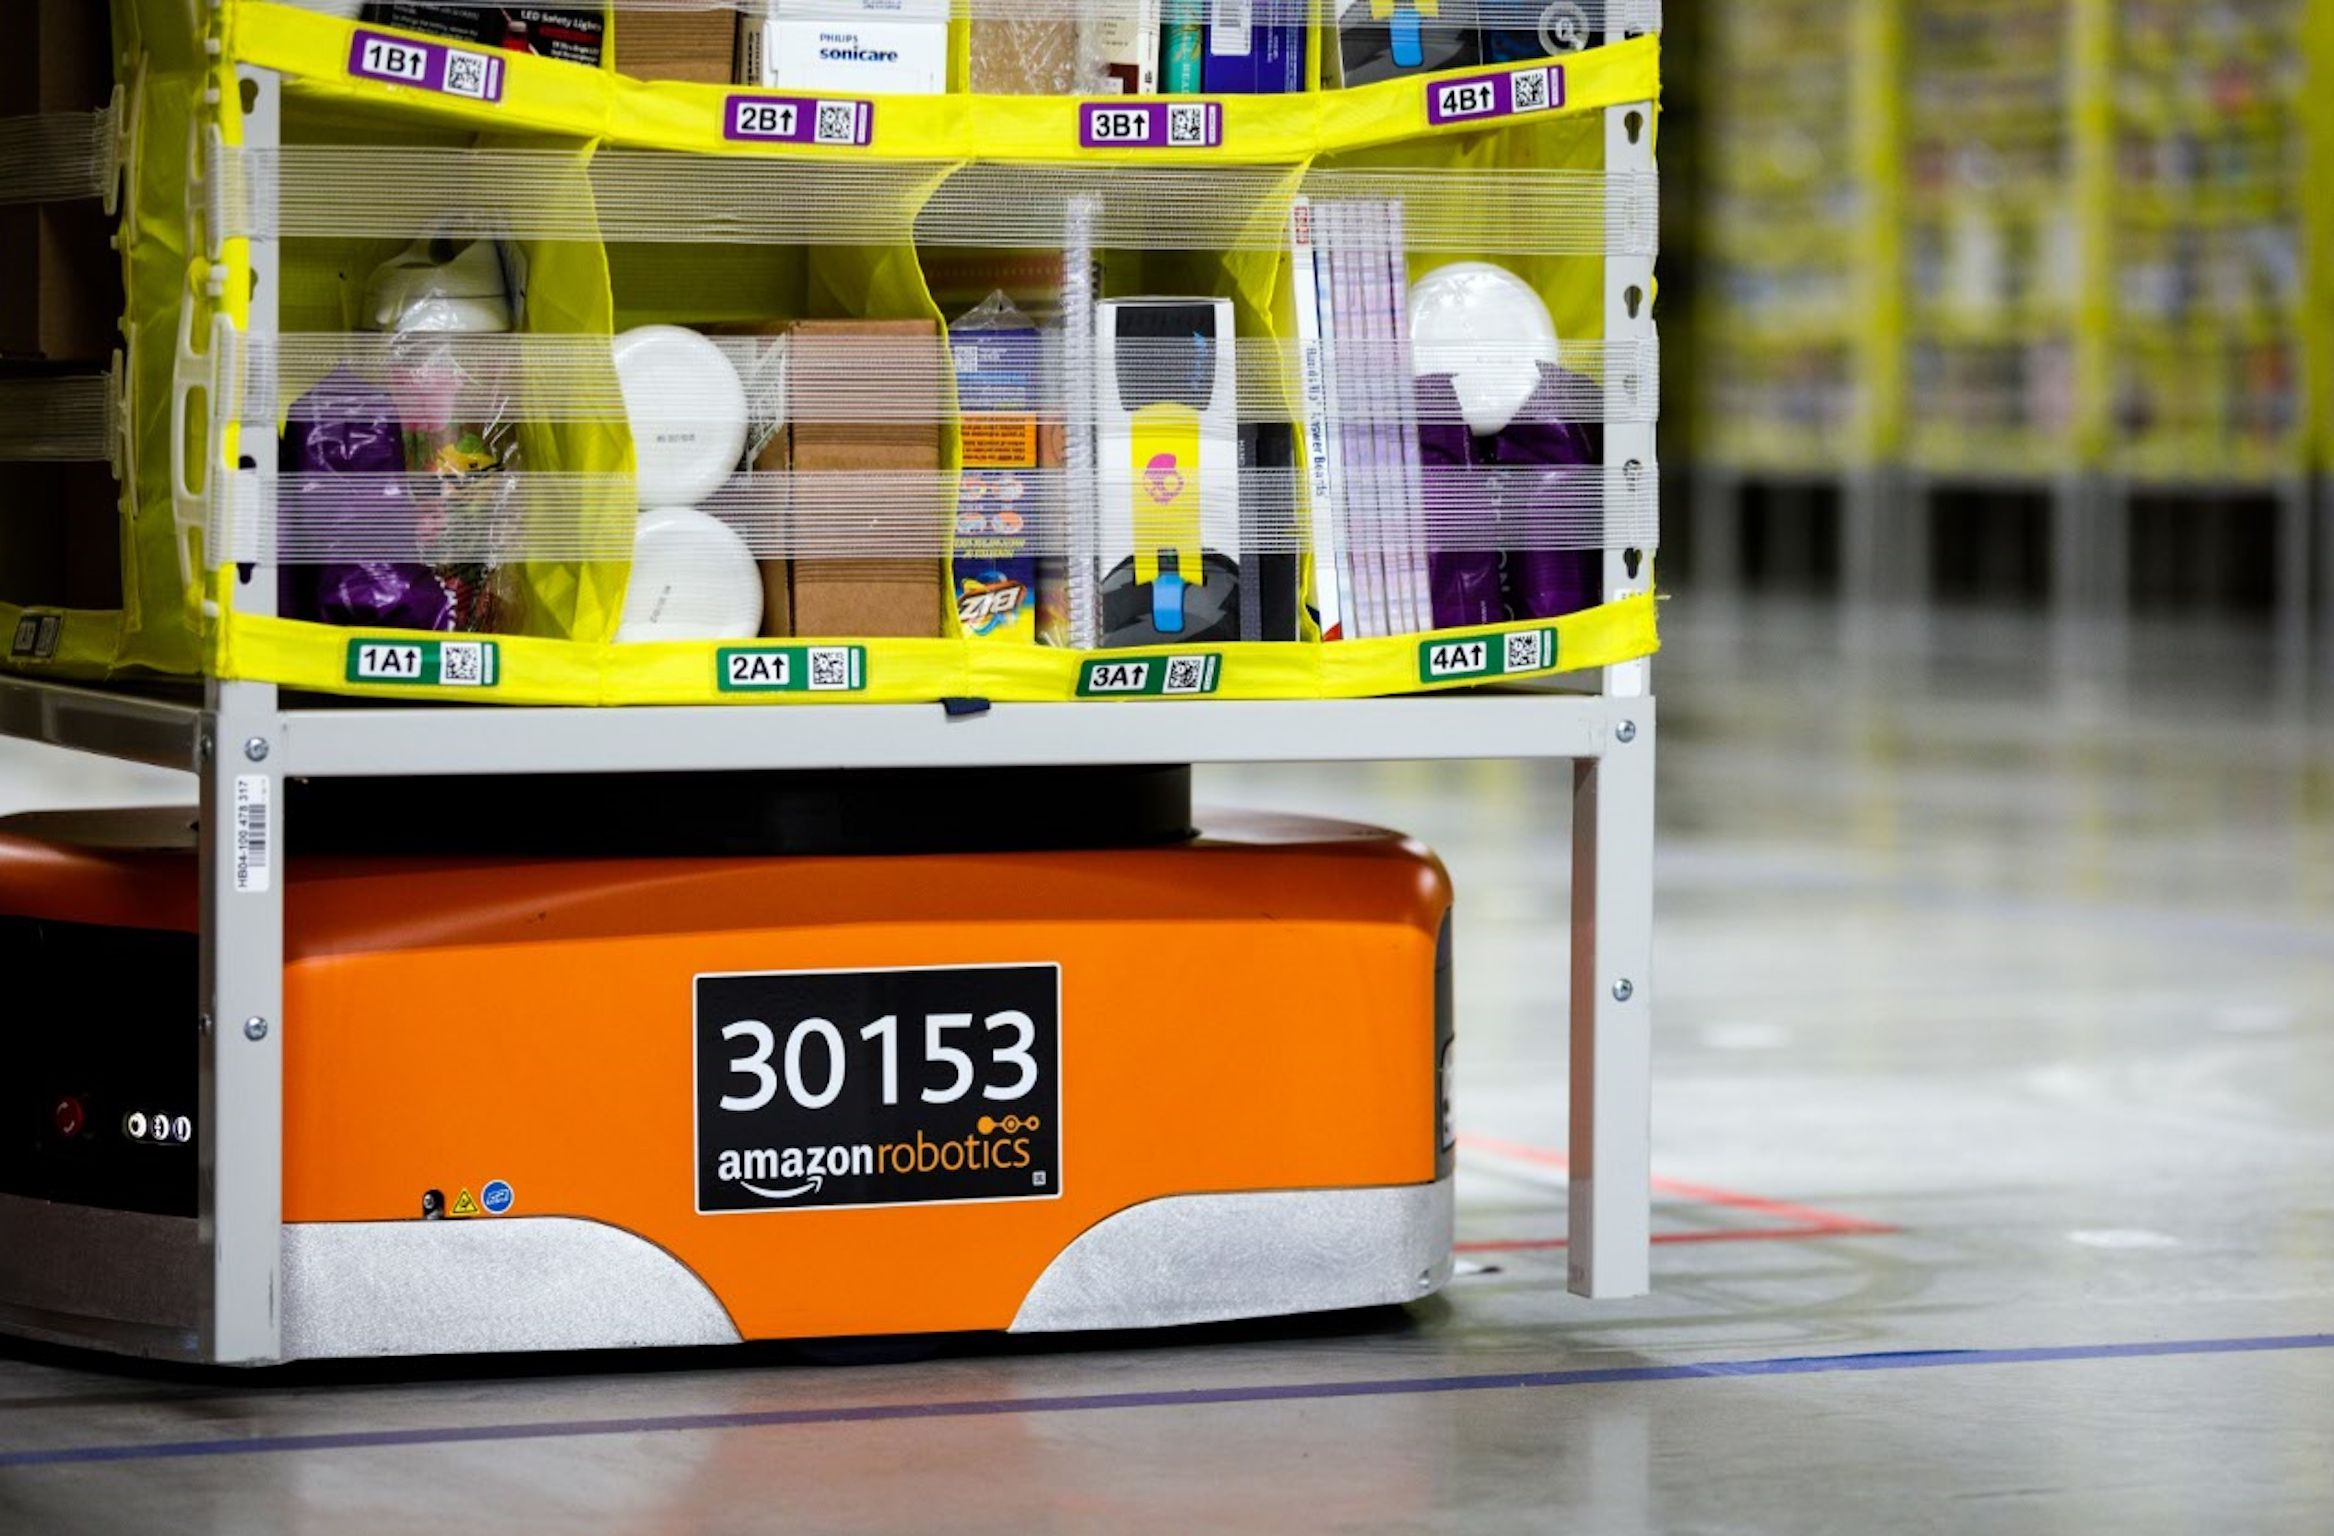
\includegraphics[width=0.6\linewidth]{figures/Amazon_Warehouse.jpeg}
    \caption{Kiva system operating in Amazon warehouse\protect\footnotemark. }
    \label{fig:Amazon Warehouse Robots}
\end{figure}
\footnotetext{https://spectrum.ieee.org/interview-brad-porter-vp-of-robotics-at-amazon}

\textbf{MAPF algorithms have broad prospects for use}.
\begin{itemize}
    \item \textbf{Warehouse Automation}: Pick-pack-and-ship system in warehouse (like Fig \ref{fig:Amazon Warehouse Robots}). Delivering items in sorting station \cite{Warehouse_Automation1,Warehouse_Automation2}.
    \item \textbf{Intersection Management}: Coordinate autonomous vehicle movement through intersections \cite{Intersection_Management}.
    \item \textbf{Robot Fleet}: Automating fleets of autonomous robots like forklift fleets \cite{Fork_Fleet1,Fork_Fleet2}.  
    \item \textbf{Agents in video games and CGIs}: Flock simulating and animating\cite{Flocking_1,Flocking_2}.
    \item \textbf{Swarm Robots}: Controlling self-organised robot swarms\cite{Swarm_Robotics}.
\end{itemize}

In general, the application of this algorithm is very broad. Furthermore, in the context of Industry 4.0 and flexible manufacturing, it has even better prospects for application\cite{Industry_41,Industry_42,Industry_43}, as centralized control is gradually becoming inadequate to meet new production needs.
 % standard chapter format
%%%%%%%%%%%%%%%%%%%%%%%%%%%%%%%%%%%%
\chapter{Literature Review} 
\label{chap:Literature_Review}
%%%%%%%%%%%%%%%%%%%%%%%%%%%%%%%%%%%%
\comment{
Use your literature review to help the reader to understand the value and the interest in your project.  You should look for related works already published that either support the merit of your project, or provide the background understanding/information to make your new claims.  Try to avoid writing a "catalogue" of related works (e.g this would have little of your own insight added).  Instead, describe to the reader why the related work is interesting or relevant to your own work.  What did they achieve?  What did they overlook?  It is highly recommend you finish your Literature Review with a final subsection "Summary", where you may wish to formulate highly specified research questions or hypotheses, or assert the need for your Research Methodology (next chapter).  

introduction
literature review
implementation
research methodology
results




\section{This is a section}
\subsection{This is a subsection}
\subsubsection{This is subsubsection}

%%%%%%%%%%%%%%%%%%%%%%%%%%%%%%%%%%%%
% Figure with subfigures
%%%%%%%%%%%%%%%%%%%%%%%%%%%%%%%%%%%%

\begin{figure}[htb]
\centering
\begin{subfigure}[t]{.5\textwidth}
  \centering
  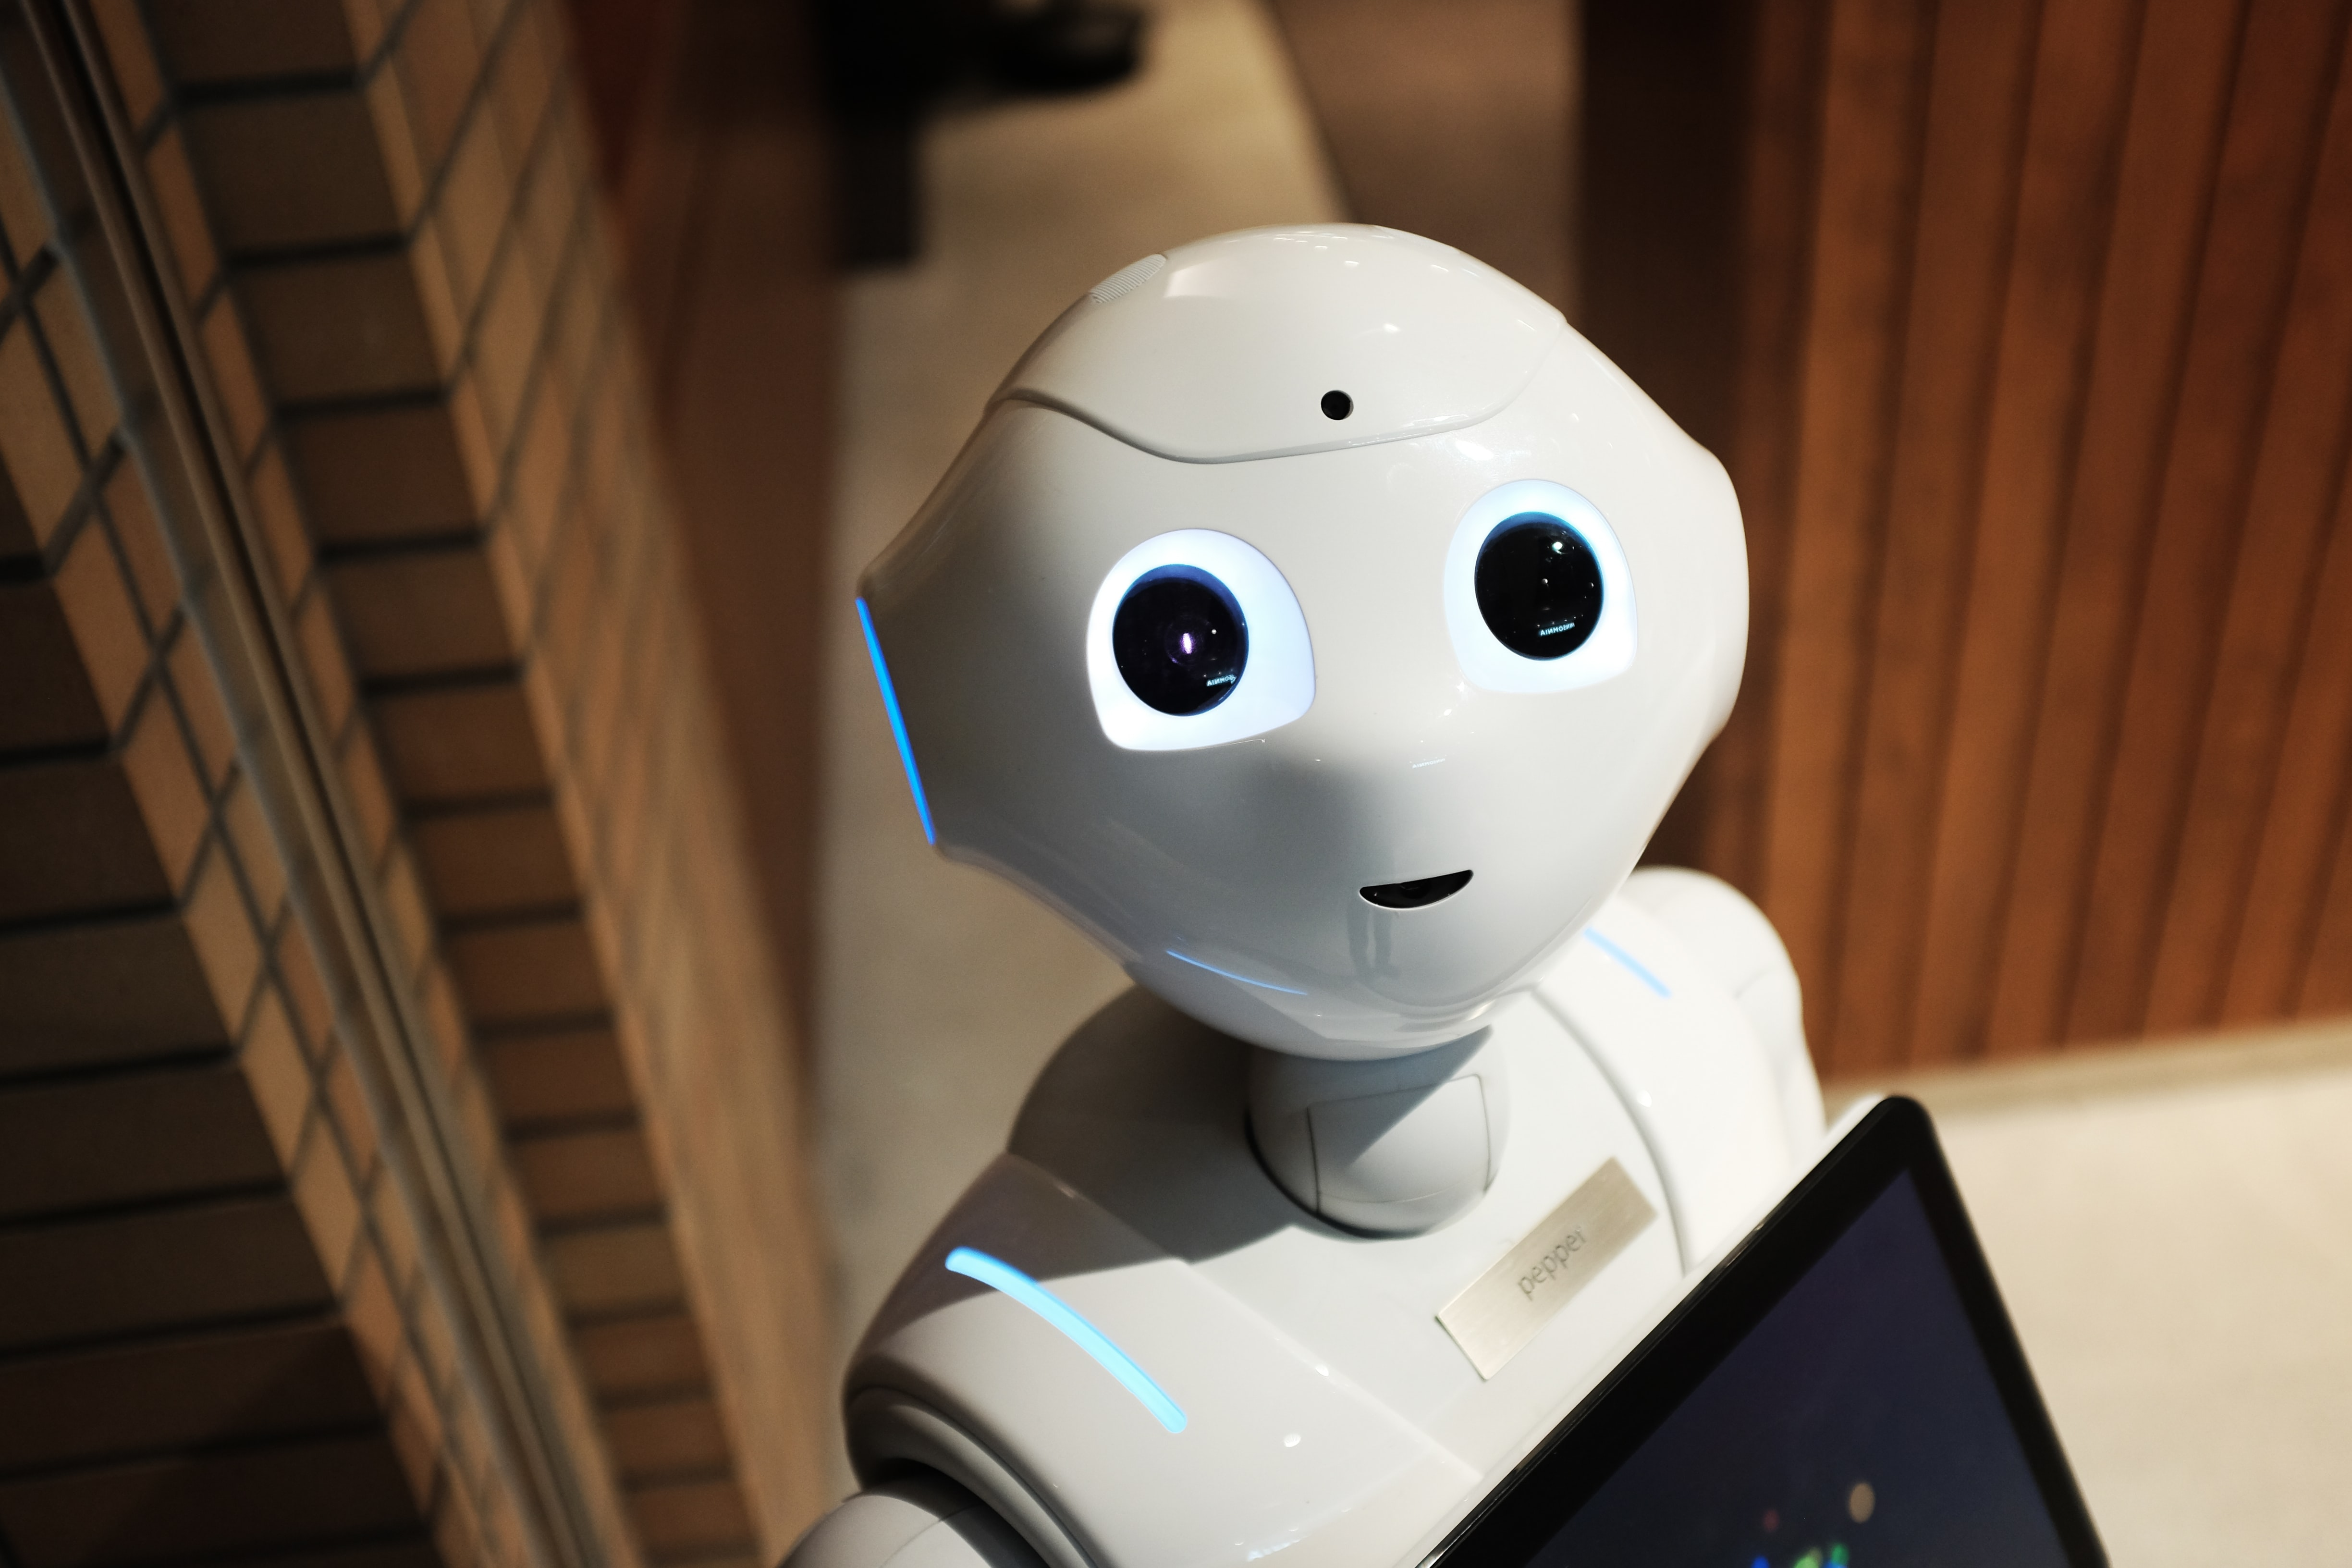
\includegraphics[height=4.5cm]{figures/Robot_1.jpg}
  \caption{\label{fig:left_robot} This is a robot.}
  \label{fig:theoretical}
\end{subfigure}%
\begin{subfigure}[t]{.5\textwidth}
  \centering
  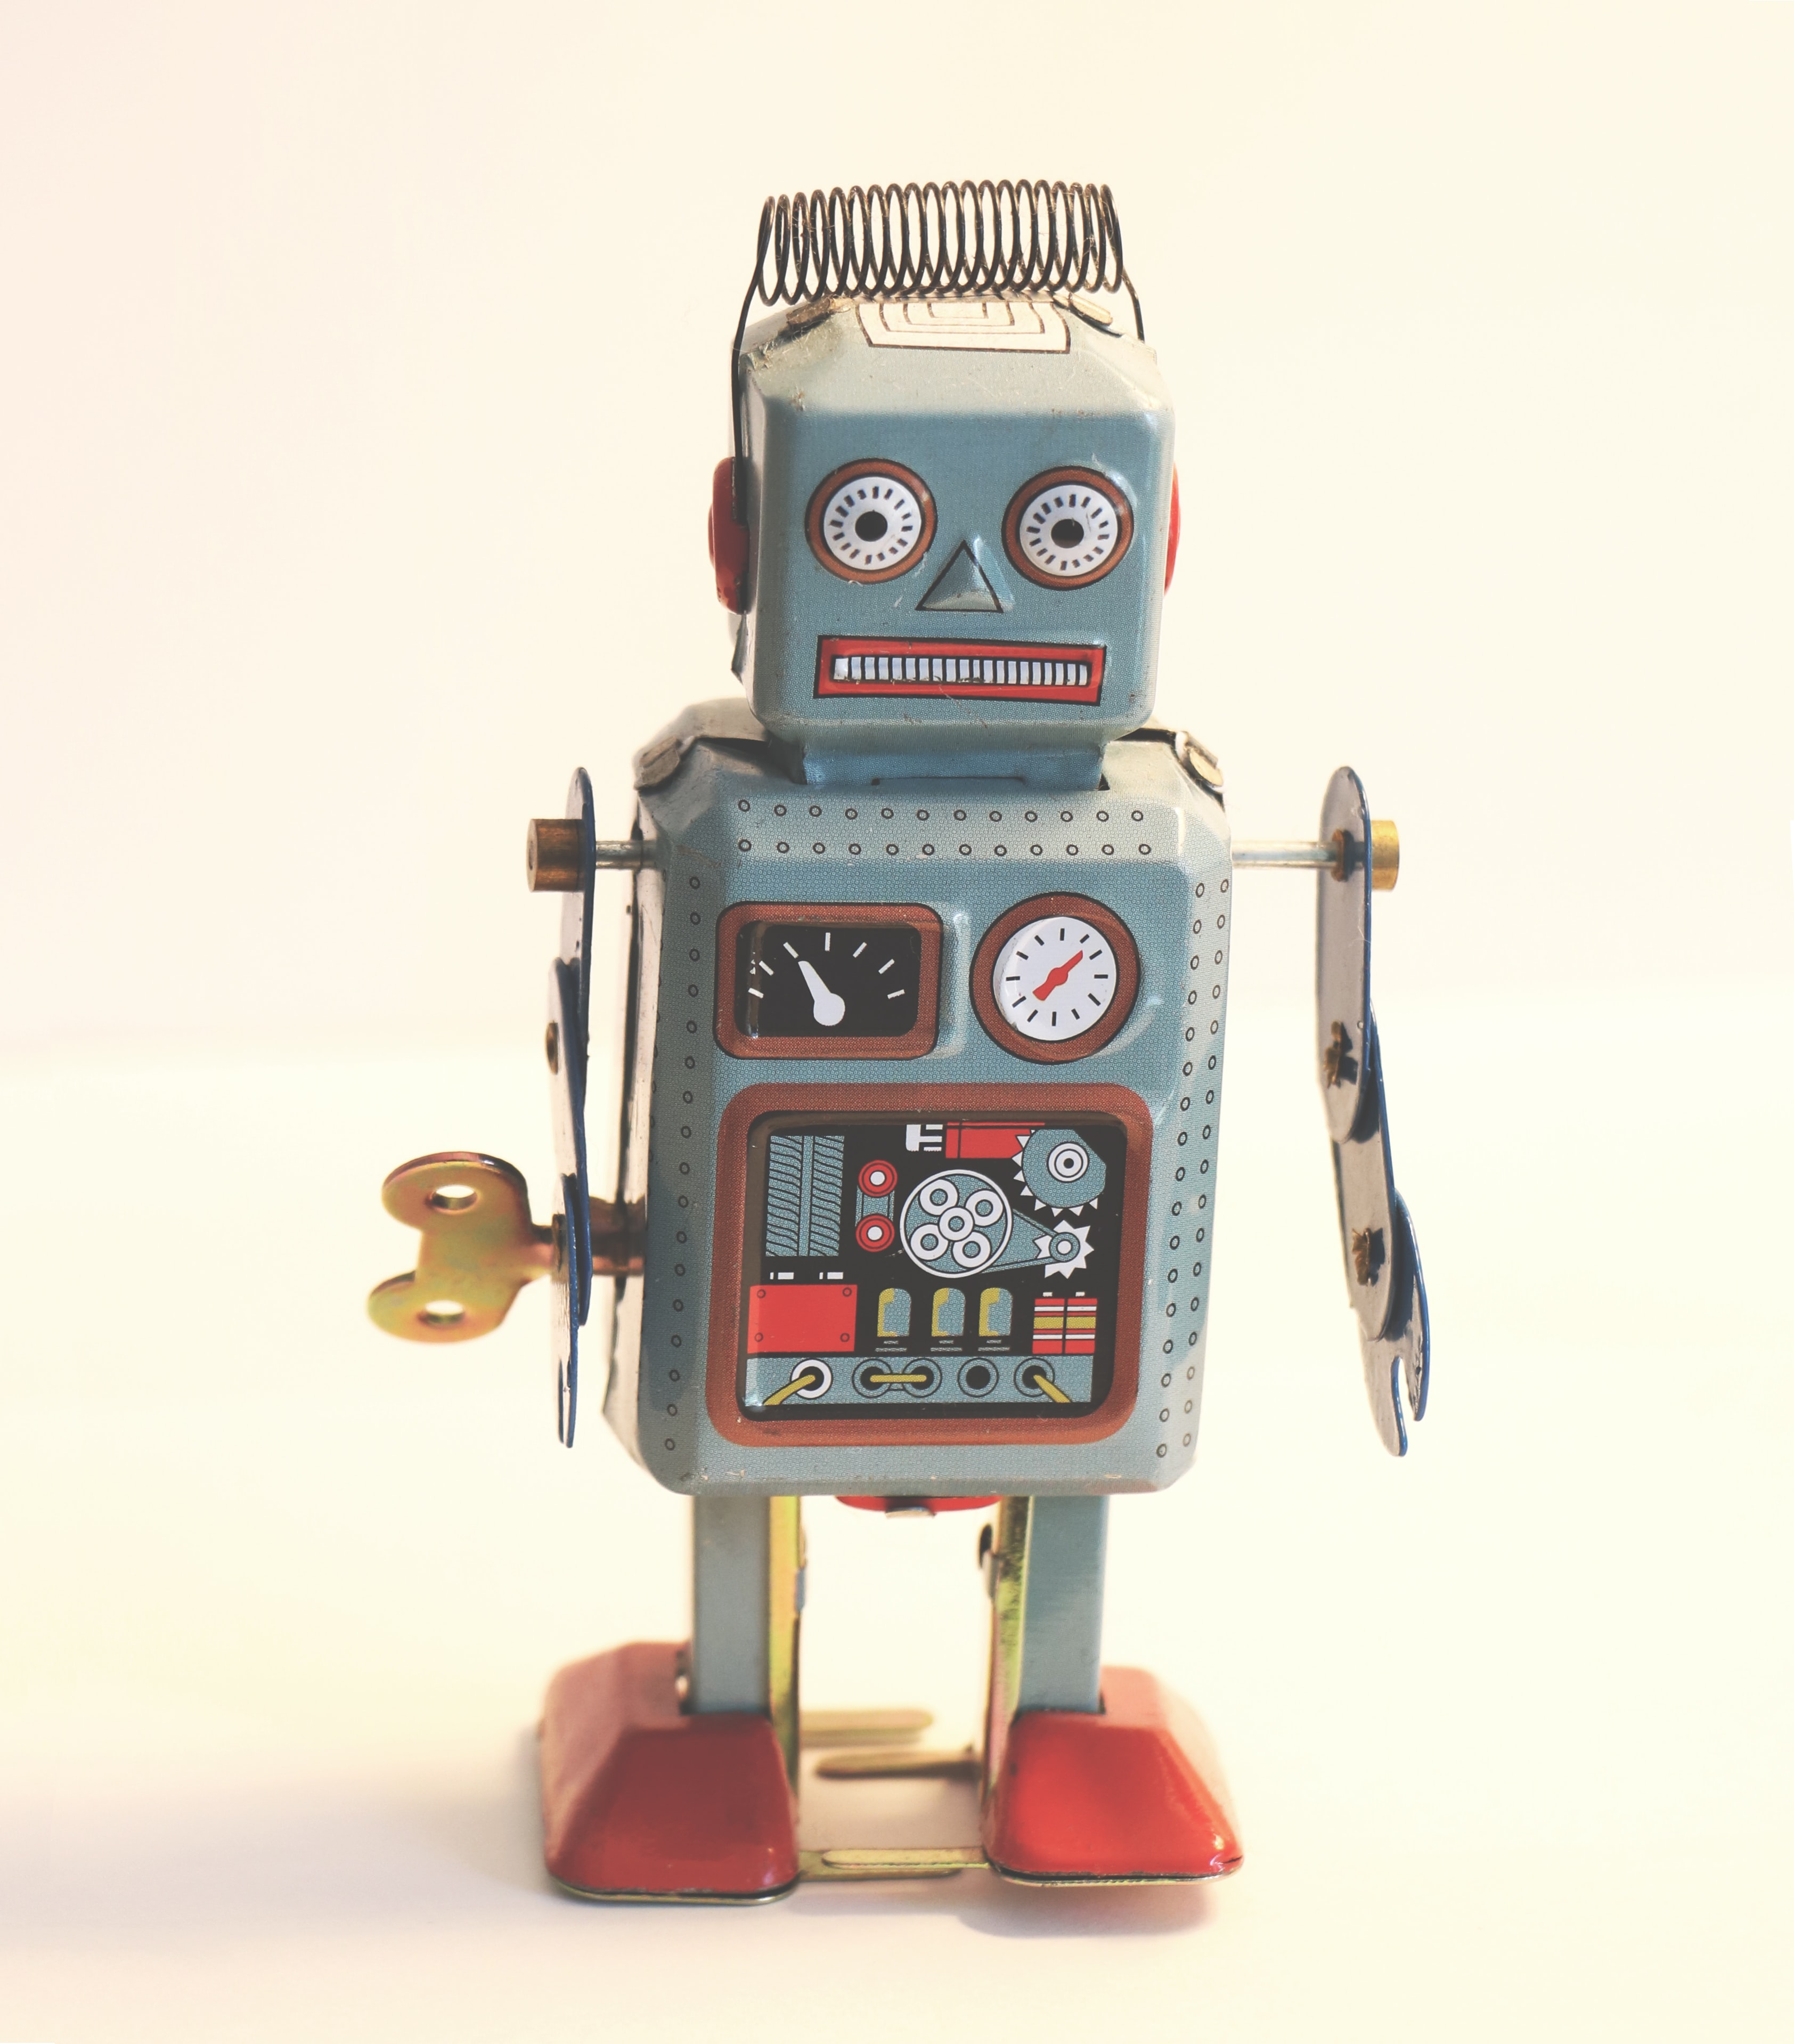
\includegraphics[height=4.5cm]{figures/Robot_2.jpg}
  \caption{\label{fig:right_robot} This another robot.}
  \label{fig:practical}
\end{subfigure}
\caption{\label{fig:two_robots} These are two robots}
\label{fig:test}
\end{figure}

For example, \cite{Robots2020} discusses the two robots depicted in Figure \ref{fig:two_robots}. There is a robot in Figure \ref{fig:left_robot} and another robot in Figure \ref{fig:right_robot}.

}

This section will provide the details of the STDMA\cite{STDMA} protocol and a review of the related \textit{Distributed Model Predictive Control} (DMPC) algorithms.

\section{STDMA Explained}

As previously mentioned in Section \ref{chap:Brief Introduction}, STDMA stands for \textbf{\textit{Self-organised Time-Divided Multiple Access}}, and it allows multiple agents to share the same channel for communication without centralised control.
The main assumtion of this protocol is that all agents have synchronised clocks. In practice, this is achieved through GPS\cite{STDMA_GPS}.

\textbf{The core idea of STDMA could be summarised as follows}: Represent continuous time with repeating frames that are consisted of discrete time slots.
While agents are always listening to messages from the channel, they look for free slots to occupy, and therefore use the occupied slots to broadcast their own data.

Agents using STDMA have \textbf{four phases}, which are arranged in chronological order as follows:

\begin{enumerate}
  \item \textbf{Initialisation}: Agents in this phase have not yet joined the network. The device listens to an entire frame and determines current allocation of each slot.
  \item \textbf{Network Entry}: Randomly choose an unallocated slot to broadcast their existance and reserve one slot for the next phase.  If the message sent didn't collide with others (i.e., only one agent which is myself choose to use this slot for entering), then the entering is successful. If the entering failed, reverse to the previous phase.
  \item \textbf{First Frame}: Use the slot reserved in the previous phase to reserve more slots for themselves. The number of reserved slots depends on the size of the data packet that the agent needs to send in each frame.
  \item \textbf{Continuous Operation}: Use the previously reserved slots to work normally. If some slots are released or more slots are needed, reapply for slots.
\end{enumerate}

Although the description above omitted some details (such as slot choosing strategy, calculation of required number of slots, etc.), it is clear that \textbf{the core idea of STDMA is the strategy of finding and reserving unallocated slots}.

This protocol also has several limitations, such as: \textbf{(1)} Collision in entering: In the Network Entry phase, multiple agents may accidentally choose the same unallocated slot for entering and broadcast their existance. \textbf{(2)} Capacity: When slots are not enough, conflicts would inevitably occur. 
There are some studies \cite{STDMA_improv1,STDMA_improv2} that proposed improvements for its limitations, but improving STDMA is not the focus of this project.

For detailed implementation, please see \textbf{PLACEHOLDER}.

\section{Distributed Model Predictive Control}

This section would cover:
\begin{itemize}
  \item An brief introduction to DMPC.
  \item Why is DMPC related to this project.
  \item A summary of related latest research developments.
\end{itemize}

\subsection{Brief Introduction}
\subsubsection{What is Model Predictive Control\cite{MPC_Review1}?}

\textit{Model Predictive Control} or MPC is a form of control that based on the model and the online prediction of the controlled system.

MPC achieves its control objective by optimising the predicted outcome of the model of the controlled system\cite{MPC_Review1}.
\textbf{On every sampling instant}, a typical MPC controller would \textbf{use the current state of the plant as initial state}, and \textbf{solve a finite-horizon open-loop optimal control problem in real-time speed}, then \textbf{apply the first step of the generated control sequence} as the next control action.

The major challenge confronting the MPC algorithm is the stability issue, with several factors contributing to this problem, such as inadequate terminal conditions and limited prediction horizons.

MPC has been extensively studied and is a widely used control algorithm\cite{DMPC_Review1}. 
It's primarily employed in fields such as process industry, power electronics, building climate and energy management, and manufacturing\cite{MPC_Applications1, MPC_Applications2}.

\subsubsection{What is Distributed Model Predictive Control? \cite{DMPC_made_easy}}

% 当系统的规模达到一定大小的时候,单一的中心化MPC控制器就不能完成控制任务了(计算要求过高/只能向有限的邻居发送数据等)。所以需要DMPC:


In many scenarios, centralised controllers fail to perform control tasks due to reasons such as the computational load increasing with the expansion of system scale, 
resulting in the controller's inability to complete real-time computations, 
or the inability to dispatch control information to all components of the system within a specified time. 
In summary, \textbf{the limitations of centralised controllers made them incapable of meeting the needs of many control scenarios}, and that is why we need distributed control.

For \textit{Distributed Model Predictive Control} or DMPC, a large system is decomposed to numerous subsystems, and each of them:
\begin{itemize}
  \item Has its own dynamic.
  \item Has an MPC controller to control its actions (predict finite future states and choose the optimal current move).
  \item Could interact with and be influenced by other subsystems (usually described as \textit{variables} and \textit{constraints}).
\end{itemize}


DMPC algorithms have the following \textbf{key characteristics}, which can help readers to understand the algorithms and distinguish one algorithm from another:

\begin{itemize}
  \item \textbf{Architecture}: Different relationships between local MPC controllers. \textbf{Hierarchical}: The entire system is divided into layers, each containing several subsystems with MPC controllers, and there exists a hierarchical relationship between these layers. \textbf{Decentralised}: Each local MPC controller controls the local subsystem and don't communicate with each other. \textbf{Distributed}: Local MPC controllers cooperate to find better solution for the overall system.   
  \item \textbf{Local - Global}: How much do the local controllers know about the overall system information.
  \item \textbf{Selfish - Cooperative}: Whether the local controller only optimizes its own cost.
  \item \textbf{Iterative - Non-Iterative}: Whether the control strategy is generated through exchange and iteration among multiple local controllers.
  \item \textbf{Serial - Parallel}: Whether the local controllers transmit their messages in a specific order or multiple controllers could communicate with each other at the same time.
  \item \textbf{Synchronised - Asynchronised}: Whether the local controllers follow a shared schedule for computation and communication. 
\end{itemize}

The advantages and disadvantages of DMPC both stem from its decentralised nature. 
Like many other decentralised algorithms, \textbf{DMPC has better scalability and robustness}, can bypass communication bottlenecks, and to some extent, allows for parallel processing.
But \textbf{coordination among multiple controllers can be quite complex},
e.g., all local controllers tend to achieve Nash equilibrium for themselves, but such a tendency may not contribute to reaching Pareto optimality and might even be counterproductive for the entire system\cite{Nash_Equi}.

\subsubsection{Why is this project related to DMPC?}

The designed algorithm (detailed explanation please see Section \textbf{PLACEHOLDER}) in this project allows each agent to:
\begin{itemize}
  \item Create and join a self-organised serial communication channel.
  \item Determine the time window for planning and plan broadcasting.
  \item Use the shared channel to broadcast its own moving plan.
  \item Receive plans of other agents and use the received information to its own movement.
\end{itemize}

Which means, the presented algorithm could be classified as a DMPC algorithm, and the problem it solves could be treated as a DMPC problem.

\subsection{Latest Researches of DMPC}



%%%%%%%%%%%%%%%%%%%%%%%%%%%%%%%%%%%%
\chapter{Algorithm}
\label{chap:Algorithm}
%%%%%%%%%%%%%%%%%%%%%%%%%%%%%%%%%%%%

\comment{

The Methodology section should provide a clear explanation of the research approach.  You want your reader to agree that you carefully considered your method so that we can trust your results to be both insightful (\underline{mean something}) and credible (\underline{not subject to error}):
\begin{itemize}
    \item A clear description of the methodology, how it creates a scientific investigation and operates to collect meaningful data.
    \item A clear justification of \underline{why} you have chosen this particular approach.
    \item Information needed for a reader to understand \underline{how} you did it (can a reader \underline{reproduce} your work, and collect equally valid results? e.g. hardware/software used, configuration, number of trials, any procedures used, etc.)
    \item A description of any approaches taken to process collected data, e.g. metrics are used to combine data in a meaningful way - you should state any used explicitly, their utility, their suitability to your methodology and their limitations.  
\end{itemize}



As on can see in Table \ref{tab:Table_with_numbers} there are numbers involved. 

%%%%%%%%%%%%%%%%%%%%%%%%%%%%%%%%%%%%
% If you have more complex tables you can 
% get a corresponding LaTeX code here
% https://www.tablesgenerator.com 
%%%%%%%%%%%%%%%%%%%%%%%%%%%%%%%%%%%%
\begin{table}[h!]
\centering
 \begin{tabular}{|c | c | c | c|} 
 \hline
  Frame number & User 1 state & User 2 state & Resulting state \\ [0.5ex] 
 \hline
 \hline
  n & 0 & 0 & 1 \\ 
 \hline
  n+1 & 0 & 1 & 2\\
 \hline
  n+2 & 1 & 0 & 3 \\
 \hline
  n+3 & 1 & 1 & 4 \\
 \hline
\end{tabular}
\caption{\label{tab:Table_with_numbers}An example of a table.}
\label{table:example}
\end{table}

For example, if $x>0$ then we can write
\begin{equation}
\label{eq:sum}
\sigma =\int_{x=0}^{\infty} \frac{1}{x^2}dx \quad ,
\end{equation}
where $\sigma$ is the integral (see Equations \ref{eq:sum}).  

}

This section provides detailed information on algorithm and its implementation.

\section*{Environment}

\begin{itemize}
    \item \textbf{Hardware:} ROG Zephyrus M16 Laptop
    \begin{itemize}
        \item CPU: 11th Gen Intel(R) Core(TM) 17-11800H @ 2.30GHz
        \item GPU: NVIDIA GeForce RTX 3060 Laptop GPU (unrelated to the experiment, information provided just for content completeness)
    \end{itemize}
    \item \textbf{Software:}
    \begin{itemize}
        \item OS: WSL2 (Ubuntu 22.04 LTS) in Windows 11 23H2
        \item Implementation Platform: ROS2 Humble, all codes written in python
    \end{itemize}
\end{itemize}

\section{Communication with STDMA}

% 这是算法的第一部分:agent间的自组织通讯
This is the \textbf{first part of the algorithm: self-organised communication between agents}.

In STDMA, agents share a single channel by autonomously determining the serial speaking order.
The approach to determining the speaking order involves agents independently assigning the right to use available time slots within the channel.

\subsection{Synchronised Clock}

% STDMA假设agent之间拥有同步时钟。
\begin{quotation}
    \textbf{Assumption 1}: 
    Agents have synchronised clocks. 
\end{quotation}

% 在实际中,同步时钟一般用GPS实现。在本文的模拟中,用一个ROS2publisher和一个topic来实现。
In practice, the synchronised clock is typically implemented with GPS. 
In the implemented simulation of this paper, it's achieved using a ROS2 publisher and a topic.
% 一个专用的ros2节点定时翻转其成员bool值,并在每次翻转此值时将翻转后的bool值publish到时钟topic中,这样在时钟topic中来形成一个占空比为50%的方波时钟信号。
A dedicated ROS2 node periodically toggles its member boolean value and publishes this boolean value to the clock topic each time it's toggled. This creates a square wave clock signal with a 50\% duty cycle in the clock topic.
% 其他普通agent通过订阅时钟话题的方式来获得同步时钟信号。
Agents obtain the synchronised clock signal by subscribing to the clock topic.

% 信道时间的离散化
\subsection{Discretisation of Channel Time}

% agent将一个完整的时钟信号周期视作一个slot,将若干slot视作一帧。
Agents consider a complete clock signal cycle (a high and a low) as one slot and consider a specific number of slots as a frame.
Time frames continuously cycle, providing a continuous and reusable slot resource for agents to use.


\begin{quotation}
    \textbf{Assumption 2:} 
    The number of slots in a frame is predefined within the agents, and this parameter value is the same for all agents.
\end{quotation}

% 注意,不要求各agent的帧起始点相同,允许agent有不同的agent起始点offset

Please note that it is not necessary for each agent to have the same starting point for their frame. 
In other words, agents are permitted to have different frame starting point offsets.

% agent在槽的正中央发送消息。
The exact middle of each slot is the timing for message transmission.
This divides a slot into two parts: before sending the message and after sending the message.

\subsection{State Machine for Channel Allocation}

% 使用STDMA的agent有四个阶段,每个阶段对应一个在网络中的状态。因此,agent加入网络的过程可以用状态机来管理,随着状态逐步转化,agent逐步加入网络并获得自己的槽
Agents employing STDMA go through four phases\cite{STDMA}, with each phase representing a stage in an agent's integration into the network. Consequently, a state machine can effectively manage the process of an agent joining the network. Through progressive state transitions, the agent incrementally integrates into the network and secures its slot.

\textbf{ADD PIC HERE} % 绘制一个槽,槽中agent发信,槽末agent数数

% 本文中对此状态机的实现如下:
The implementation of this state machine in this paper is as follows:

\begin{enumerate}
    \item \textbf{Listening}
    
    % 在此状态下的agent如何如何如何

    % 此状态下的agent的目的是确定当前的信道槽位分配情况,此状态下的agent尚未进入网络
    In this state, the agent's objective is to determine the current channel slot allocation by 'Listening' to the channel. 
    Agents in this state have not yet joined the network.

    Slot allocation determination: In a slot:
    \begin{itemize}
        % 如果仅收到一条消息:槽有主
        \item If only one message was sent: the slot is occupied by the sender.
        % 如果收到多条消息
        \item If multiple messages were sent or no message was sent: the slot is considered free.
    \end{itemize}

    The initial state of an agent is this state.

    % Transition Condition: 每次听完完整的一帧后,agent尝试离开此状态
    \textbf{Transition Condition}: After listening to a complete frame, the agent attempts to exit this state.
    \begin{itemize}
        % 当信道中有一个或多个未被使用的槽时,进入entering状态
        \item $\rightarrow$ Entering: There are one or more unoccupied slots within the frame.
        % 信道中无空闲槽时:呆在listening.
        \item $\circlearrowleft$ Listening: There are no free slots remaining in the frame. This suggests that the channel's capacity has been fully utilized, and the agent can only stay 'Listening' and remain idle.
    \end{itemize}
    
    \item \textbf{Entering}
    
    % 在此状态下的agent的目的是如何,agent的状态是如何
    In this state, the agent attempts to occupy a free slot in order to try 'Entering' the network.

    % Transition Condition: 
    \textbf{Transition Condition}: 
    % Agent尝试占用一个随机的在lisening状态中确认的free slot.
    The agent tries to occupy a random free slot that was identified during the 'Listening' state. 
    % 在这一槽中,agent发送其id,来尝试获得此槽
    Within this slot, the agent \textbf{transmits its unique ID} in an effort to occupy the slot.

    \begin{itemize}
        \item $\rightarrow$ Checking: The agent transitions to the 'Checking' state immediately after sending the occupation attempt message.
    \end{itemize}


    \item \textbf{Checking}
    
    % 在此状态下的agent的目的是如何,agent的状态是如何
    % 此状态下的Agent刚刚在某一槽中发布了一条信息,需要根据槽内收到的消息的数量判断自己对此槽的所有权。
    In this state, the agent has just broadcast a message in a specific slot and must ascertain its ownership of that slot, based on the quantity and content of messages received within it.
    % 通过检查自己对此槽的所有权,变更自身状态。
    By 'Checking' its ownership of that slot, the agent transits its state.

    % 注意,未进入网络和已进入网络的agent都会在发布消息后进入此状态。
    Note that both agents that have not yet entered the network and those that have will transition to this state after sending a message.

    % Transition Condition:
    \textbf{Transition Condition}: Transition the state based on the number of messages received in the slot where a message has been sent.
    \begin{itemize}

        % 如果只收到一条消息且来自自己:说明自己拥有此槽位,即在网络中
        \item $\rightarrow$ In: If only one message is received and it's from itself, it indicates that the agent has ownership of that slot, meaning it is 'In' the network.
        % 任何其他情况:自己不拥有此槽位,重新尝试获得槽位。
        \item $\rightarrow$ Listening: In any other situation: The agent does not have ownership of that slot and should try to secure a slot again.
        
        % 解释:所有其他情况包含:
        Explanation: All other situations include:
        \begin{itemize}
            % 没有收到自己的消息
            \item Didn't receive its own message: This suggests that either the broadcast was unsuccessful or the reception was unsuccessful (e.g., due to hardware damage or scheduled broadcasting being prevented, etc.). In both situations, we do not want the agent to enter the network, as its communication function may not be consistently reliable.
            % 多个节点尝试在同一槽内发送消息:
            \item Multiple agents sent messages within one slot (i.e. collision):
            
            % 碰撞情景1:多个正在进入网络的agent恰好选择了同一个槽位。此种碰撞在本算法框架下无法避免,但由于仅发生在未进入网络的agent之间,对其他有效通讯没有影响。
            Collision Scenario 1: Multiple agents attempting to join the network coincidentally select the same slot. While such collisions are unavoidable within the context of this algorithm, they only occur among agents that have not yet entered the network and thus do not impact other normal communications.
            
            % 碰撞情景2:已加入网络的agent与未加入网络的agent发生碰撞。此种碰撞在理论上是不应该发生的,因为未加入网络的节点应当只尝试获得未被使用的槽位。若agent错过了时钟脉冲,则可能会出现此种情况。若某agent失去时钟脉冲,则会导致其和所有其他agent失去同步,进而导致事故。这一情况要尽可能避免。
            Collision Scenario 2: A collision occurs between an agent that has already joined the network and one that has not. In theory, this type of collision should not occur, as agents not yet in the network should only attempt to occupy unoccupied slots. However, this situation may arise if an agent misses a clock pulse. Missing a clock pulse can cause an agent to fall out of synchronization with all other agents, potentially leading to conflicts and accidents. Efforts should be made to prevent this situation as much as possible.
        \end{itemize}

    \end{itemize}    


    \item \textbf{In}
    
    % 在此状态下的agent的目的是如何,agent的状态是如何
    % 在此状态下的agent已经进入网络,且应当始终在网络中,直到其通过停止定期发送消息来放弃其槽位。
    In this state, the agent is 'In' the network and should stay in the network until it relinquishes its slot by stopping its regular message transmission.
    
    % Transition Condition:
    \textbf{Transition Condition}:
    \begin{itemize}
        % 每次发送消息后,检查自己对此槽的所有权
        \item $\rightarrow$ Checking: After publishing a message, verify ownership of that slot.
    \end{itemize}

\end{enumerate}

\textbf{ADD PIC HERE} % 画一个状态机的图片 

\subsection{Summary}

% 实现了agent的自组织无碰撞信道分享。信道的时间被表示为包含指定数量槽的重复的帧,
% agent通过尝试占有帧中一个槽的方式来加入网络,此过程由状态机管理并实现。
This achieves agent self-organization and collision-free channel sharing. The channel's time is represented as repeating frames containing a specified number of slots. An agent attempts to join the network by trying to occupy one slot within a frame, the joining process is managed and implemented by a state machine.

\section{Path Planning and Sharing}


% agent的移动模型, 计划的作用,分享的方式
\subsection{Planning Framework and Definition}


\subsubsection{Map}
The map is a grid world with obstacles, and:
% 本文中所使用的地图仅包含静止障碍物
\begin{quotation}
    \textbf{Assumption 3}:
    % 所有的障碍物都是静止的
    All obstacles in the map are stationary.
\end{quotation}

\subsubsection{Agent Capabilities and Constraints}

\textbf{Capabilities}:
\begin{itemize}
    % 每时间步可以不动或移动一格
    \item Agents can choose to either remain stationary or move to an adjacent non-diagonal grid cell at each time step (corresponding to a slot in the STDMA section).
    % 可以完美执行计划
    \item Agents can execute their own plans with complete accuracy.
\end{itemize}

\begin{quotation}
    \textbf{Assumption 4}: 
    % agent的移动不受外部扰动的干扰,且对自己运动的预测百分之百准确。
    The agent's movement is not affected by external disturbances, and its prediction of its own motion is completely accurate.
\end{quotation}

\textbf{Constraints}

\begin{itemize}
    % 不能碰撞
    \item Agents should not collide with each other.
    % 不能穿墙
    \item Agents should not use positions on the map that are occupied by obstacles.
\end{itemize}

\subsubsection{Collision Definition}

% 在本文中,以下两种情形被视为碰撞:
In this paper, the following two scenarios are considered as collisions:
\begin{itemize}
    % 两个或以上节点在同一时刻位于地图上的同一2D位置
    \item Two or more agents are located at the same 2D position on the map at the same time.
    % 两个节点交换位置。即,t时刻agentA位于位置a,agentB位于位置b,t+1时刻A位于b,而B位于A
    \item Two agents swapping their positions. That is, at time $t$, agent $A$ is at position $a$, and agent $B$ is at position $b$. At time $t+1$, agent $A$ is at position $b$, while $B$ is at position $a$.
\end{itemize}

\textbf{ADD PIC HERE} % 放一张描述碰撞的图

\subsubsection{Plan Definition and Constraints}

\textbf{Definition}

% 计划的定义就是一串三维坐标点,其中每个坐标点都由一个二维坐标和一个时间点构成。
A plan is a sequence of 3D coordinate points. Each coordinate point comprises a 2D location and a specific time, essentially indicating both the spatial and temporal aspects.
% 由于agent mobility的约束,计划中相邻点的二维坐标部分必须为非对角的相邻点。此外,计划中的相邻点的时间点也必须是单调以1的步长递增。


% 计划的约束
\textbf{Constraints}

% 计划的约束是:1. 不能与其他agent或地图中的障碍物发生碰撞。 2. 计划中相邻的点,空间上必须是非对角的相邻点,时间上后一点必须比前一点增加1。 3. 计划的第一个点必须在空间上与开始计划时刻的agent位置位于非对角的相邻点。
\begin{enumerate}
    % 计划中的点必须符合agent的移动能力与约束
    \item The points in the plan must align with the agents' capabilities and constraints.
    % 计划中的第一个点必须是是agent开始计划时刻的位置的非对角相邻点,且满足agent的其他约束
    \item The first point in the plan must be a non-diagonal adjacent point to the agent's initial position at the start of planning, and it must also satisfy the agent's other constraints.
\end{enumerate}


% 分享
\subsubsection{Plan Broadcasting Method and Time Window for Planning}
% 分享计划的方式

\textbf{Broadcasting}

% agent通过stdma所分享的信道进行自身计划的分享,即,在每个属于自己的槽的中央在信道中广播自身的计划。
Through the channel facilitated by STDMA, agents broadcast their individual plans. This entails agents broadcasting their plans in the middle of each slot allocated to them within the channel.

% 注意,计划制订时仅生成二维坐标的序列,时间在计划过程中是隐含的。计划中的时间维度在计划被接收时由接收者自己添加。
Note that during plan formulation, only a sequence of 2D coordinates is generated, and time is implicit in the planning process. The time dimension of the plan is added by the recipient upon receiving the plan.
% 因此,每次仅传输一组二维坐标序列即可。
As a result, only a set of 2D coordinate sequences needs to be transmitted each time broadcasting.



% 计划的时机
\textbf{Time Window for Planning}

% 如前文所述,每个agent在属于自己的槽的中间发布信息。
As previously mentioned, each agent publishes their message (their plan and ID) in the middle of the slot allocated to it.
% 基于这一特性,对于每个agent来说,存在这样一个定期出现的时间窗口:涉及计划制订的所有变量都是确定的,且自己的计划只要制订完成就可以立即发布。
Based on this rule, for every agent, there exists a periodically repeating time window where all variables related to planning are constant, 
and the agent's own plan can be immediately published as soon as it is formulated.

% 这个时间窗口就是自己的槽的前半部分。在这段时间内,不会有其他agent发布新的计划,且此时段结束后就可以立即发布自身的计划。
This time window is the first half of the agent's own slot. Within this interval, no other agents will broadcast new plans, and as soon as this interval ends, the agent can immediately publish its own plan.
% 由于此窗口是一个槽,这一窗口在每一帧中会出现一次
Given that this time window is a segment within a slot, it will occur once in each frame. 

\textbf{ADD PIC HERE}% 画图解释进行计划的时机

% 模型预测和receding horizon
\subsubsection{Model Predicting and Receding Horizon}

\textbf{Model Predicting}

% 本文中通过假设agent可以绝对准确执行自身计划的方式对模型预测进行了大幅度简化。
In this paper, the model predictions have been significantly simplified by assuming that agents can execute their own plans with absolute accuracy.
% 只要自己的计划中的点满足agent的移动能力,就一定可以按时抵达目标位置。同样,其他agent的计划也是绝对准确的。
As long as the points in an agent's plan adhere to its mobility capabilities, the agent will invariably reach the planned position on time. Similarly, plans of other agents are also assumed to be entirely accurate.


\textbf{Receding Horizon}

% 在模型预测控制中,随着时间的推进,预测窗口会不断向未来推进。
Within the context of model predictive controlling, as time progresses, the prediction horizon continuously advances into the future (horizon receding).
% 本算法中,预测窗口基于以下几条规则得以推进:
Within this algorithm, the horizon advances based on the following set of rules:


% agent进入地图的流程
\subsubsection{The process of an agent entering the map}

% 由于agent在进入网络前无法发言,其存在是不被其他agent知道的。
    



\subsection{Path Planning Function and Implementation}

% 在每个计划窗口开始时,计划函数被调用,用以生成接下来agent的移动计划。
At the start of each planning window, the path planning function is called to generate the upcoming movement plan for the agent.

\subsubsection{Inputs of the function}

\begin{itemize}
    % 地图,自己的当前位置,目标点,其他agent的计划
    \item map, agent's current position, goal, plans of other agents

    % 这些是计划所需的基础信息。
    Foundational information required for the planning process.

    % 是否是第一次进入地图? 
    \item first ever plan
    
    % 这是一个bool值,指示当前计划是否为agent的进入地图时的首个计划。
    This is a boolean value that indicates whether the current plan is the first plan for the agent upon entering the map.



    % 所需计划之长度
    \item required plan length
    
    % 每次生成计划时要求生成的长度。
    The required length of the plan to be generated each time.

    % 由于agent每帧进行一次计划,而agent必须遵循其计划移动,所以每次生成的计划之长度必须至少等于一帧中slot的数量(即帧长度)。
    Since the agent plans once per frame, and the agent must follow its planned movement, the length of each generated plan must be at least equal to the number of slots in a frame (i.e., the frame length).

    % 如果agent的计划长度短于帧长度,会导致在帧末尾agent没有可使用的计划,其存在不为其他agent所知,而导向潜在的碰撞。
    If the agent's plan length is shorter than the frame length, it will result in the agent having no available plan near the end of the frame, and its presence will be unknown to other agents, leading to potential collisions.
    % 这一限制可以通过一些适当的技巧解决,如:agent之间对无计划时的移动有一些共识,进而可以用这一共识预测其他agent的行动,来允许计划长度短于两次计划之间的间隔。
    This limitation can be addressed through some appropriate techniques, such as having a consensus among agents on movement when there is no plan, which can then be used to predict the actions of other agents when their plans expire, allowing the plan length to be shorter than the interval between two planning windows.
    
    % 在本实现中,只有当终点在要求计划长度以内可达时,才会返回比要求长度更短的计划。
    In this implementation, a plan shorter than the required length will only be returned if the goal is reachable within the required plan length.
    
    % horizon
    \item predicting horizon
    
    % 算法所允许预测的horizon上限
    The upper limit of the horizon length allowed for prediction in single planning window.
    % 若一条可能路径的长度达到horizon,则本次计划中不再继续扩展此路径。
    If the length of a potential path reaches the horizon, then this path will not be further extended in the current planning session.
    
    % 这一限制主要来自于运算速度。
    This limitation mainly arises from the computational speed, and:
    \begin{quotation}
        \textbf{Assumption 6}: 
        The predicting horizon upper limit is predefined within the agents, and this parameter value is the same for all agents.
    \end{quotation}

    % 如果要求的计划长度比horizon长如何处理?对此,agent的共识是,当计划用尽时,其他agent待在原地不动。虽然待在原地不动并不是由计划生成的无碰撞行动,但是由于每次计划时,正在计划的agent所生成的计划都一定是时间上最远的(依次按顺序进行计划,每次计划都只生成固定长度),所以这一共识不会导致潜在的碰撞。
    What if the required plan length is longer than the horizon? 
    There is a consensus among agents on this: 
    when the plan is exhausted, the agent stays in place without moving. 
    Although staying in place is not a collision-free action generated by planning, 
    since every time an agent plans, the plan it generates is always the furthest in time 
    (planning in sequence, each plan only generates a fixed length), 
    so this consensus will not lead to potential collisions.
\end{itemize}

% 创建一个成员为当前位置的openset(即已发现但还未访问的点)。起点的时间维度为0(对应正在计划的这一槽)
% 当openset不为空时:
%   从openset中弹出综合代价 = 耗时+启发式代价(距终点曼哈顿距离)最低的点及其所对应的路径。
%   如果路径长度大于等于horizon:continue
%   如果此点是终点且耗时<=required length: 返回路径。
%   获得此点的可用邻居点(位于地图中可用点且不与其他agent发生碰撞,且不位于closedset的点)作为待扩展点
%   邻居点的时间戳是当前点+1。
%   若是第一次计划,则可用邻居点(下一步待扩展点)必须为起点。
%   将待扩展点推入openset中。
%   将此点推入closedset中。
% 从closedset中选出对应路径离终点的综合代价最低的,返回此路径
% 若closedset为空且agent是第一次计划:返回空。此时地图中没有足够的供其进入的空间。

\begin{algorithm}[H]
    
    %\small
    %\SetNlSty{}{}{}{}{}{}
    %\SetNlSty{textbf}{}{}{}{}{}
    \setstretch{1.1}


    \caption{Path Planning Function}
    \label{alg:path_plan}
    \DontPrintSemicolon % 不要分号
    
    \SetKwFunction{pathplan}{path\_plan}
    \SetKwProg{Fn}{Function}{:}{}
    \SetKwIF{If}{Elseif}{Else}{if}{then}{elseif}{else}{end}
    
    \Fn{\pathplan{
        map, current position (2D coordinate), goal (2D coordinate), others' plans, first plan or not, required plan length, predicting horizon
        }}{
        current position $\leftarrow$ set (current position, time = 0, cost = time + Manhattan distance (heuristic cost) of current position and goal, path = empty list)\;
        frontier $\leftarrow$ [current position]\;
        visited $\leftarrow$ set()\;
        path list $\leftarrow$ []\;
        \While{frontier}{
            current point $\leftarrow$ pop the point with the lowest cost in frontier\;
            current path $\leftarrow$ the path corresponding to the current point\;
            current time $\leftarrow$ the time corresponding to the current point\;
            \If{current path length = predicting horizon}{
                path list append current path\;
            }
            \If {current path length > predicting horizon}{
                \textbf{continue}\;
            }
            \If{current point = goal and current plan length $\leq$ required length}{
                \Return{current path}\;
            }
            \If{first plan}{
                neighbour $\leftarrow$ start of the agent\;
            }
            \Else{
                neighbour $\leftarrow$ non-diagonal neighbour points of current point\;
                }
            \ForEach{neighbour}{
                \If{(neighbour, current time+1) is not in visited and neighbour is valid}{
                    frontier append set(neighbour, time = current time + 1, cost = time + Manhattan distance of neighbour and goal, path = current path + neighobur)\;
                    add (neighbour, current time+1) to visited\;
                }
            }
        }

        \If{path list}{
            path $\leftarrow$ the plan with the last point having the smallest Manhattan distance to the goal\;
            \Return{The portion of the plan that does not exceed the required length}\;
            }
        \Else{
            \Return None
        }
    }
\end{algorithm}

% 注:上述流程意味着算法每次都冷启动,从头开始路径规划而不是继承上一次计划的剩余可用部分。这是有原因的。原因将在PLACCEHOLDER处介绍。
Note: The process described above means that the planning always starts fresh, beginning path planning anew rather than carrying over any remaining usable portions from the previous plan. The reason behind it will be explained in the \textbf{PLACEHOLDER} section.

\textbf{Output of the function}:

% 若agent当前位于地图内,则生成一个从当前点相邻位置开始的长度指定的计划。
If the agent is currently inside the map, generate a plan of the specified length starting from a position adjacent to the current position.

% 若agent不位于地图内,则尝试生成一个从指定起点开始的长度指定的计划。
If the agent is not inside the map, generate a plan of specified length starting from the specified starting point.

% 若不存在符合要求的达到指定长度的计划,则返回None。
If there is no plan meets the requirements, return None.

% 抵达终点后的行动?
\textbf{Actions after reaching the goal}:

% agent关闭自身,停止向信道中发送消息(意味着放弃自己在信道中的槽),并从地图中消失。
The agent shuts itself down, stops sending messages to the channel (meaning it gives up its slot in the channel), and disappears from the map.

\section{Summary}

% 假设:
\subsection{Assumptions:}
\begin{enumerate}
    \item Agents have synchronised clocks.
    \item All obstacles in the map are stationary.
    \item The agent’s movement is not affected by external disturbances, and
    its prediction of its own motion is completely accurate.
    \item There always exists at least one continuous 2D path in the space
    for the agent to use
    \item  The number of slots in a frame is predefined within the agents, and
    this parameter value is the same for all agents.
    \item The number of predicting horizon upper limit is predefined within the
    agents, and this parameter value is the same for all agents.
\end{enumerate}

\subsection{Implemented Functions:}

% agent启动后,自主尝试加入当前的通讯网络。加入网络后,尝试从指定起点进入地图。进入地图后,根据他人的移动计划和地图信息,不断寻找可以令自己接近终点的无碰撞连续二维坐标序列,并分享自己的移动计划。到达终点时,放弃自己在网络中的位置,停止活动。
After the agent is activated, it autonomously attempts to join the current communication network. 
After joining the network, it tries to enter the map from the specified starting point. 
Once inside the map, based on the movement plans of others and map information, it continuously searches for a collision-free continuous 2D coordinate sequence that can bring it closer to its goal, and broadcasts its own movement plan. 
When it reaches the goal, it releases its position in the communication network, exits the map and ceases activity.








%%%%%%%%%%%%%%%%%%%%%%%%%%%%%%%%%%%%
\chapter{Results}
\label{chap:Results}
%%%%%%%%%%%%%%%%%%%%%%%%%%%%%%%%%%%%



% 实验场景设置
\section{Experiment Design}

\subsection*{Map}
\label{chap:map}

% 本文中的所有实验在一张模拟库房场景的地图中进行。
All experiments in this paper were conducted on a map simulating a warehouse scenario.
% 此地图是从一组被广泛使用的benchmark中选出的。
This map was selected from a widely-used benchmark set\cite{stern2019mapf}\footnote{https://movingai.com/benchmarks/mapf.html} for testing, due to its appropriate size and obstacle distribution.

\begin{figure}[htbp]
    \centering
    \includegraphics*[width = \linewidth]{figures/map(color).png}
    \caption{The map used in the experiments. The outer border is not included in the map.}
    \label{fig:Map}
\end{figure}

% 地图的大小为161*63(外侧的框不是地图的一部分),图中的绿色代表障碍物,白色代表可通行。所有狭窄通道(边缘和障碍物之间的通道)均为一格/一像素宽。
The size of the map is 161$\times$63 (the outermost green frame is not part of the map), 
with green representing obstacles and white representing passable areas.
All narrow corridors (channels at the border and between obstacles) are one grid / pixel wide.

\subsection*{STDMA Channel Slot Duration}

% 由于agent需要在自己的槽内解出finite horizon优化问题,单个slot的时长被agent的计算能力限制。
Due to the necessity for agents to solve a finite horizon optimization problem within their allocated time slots, the duration of a single slot is constrained by the computational capacity of the agent.
% 对于本实验的环境,将slot的时长设为1秒,这最多允许agent将planning horizon设为60.
In the environment of this project (see Section \ref{chap:environment}), the duration of each \textbf{STDMA slot is set to  1 second}, allowing agents to set their \textbf{planning horizon to a maximum of 60}.

\subsection*{Agent Initialization and Behaviour}
\label{chap:agent initialisation}
\subsubsection{Starts and Goals Initialization}
% agent的起点和终点是如何生成。。。
% 生成若干起点-终点对,保存为单独的文件,每次启动实验时从此文件中依次读入起点-终点对,并依次分配给启动的agent。
The starting points and their corresponding goal points for agents are pre-generated and stored in a launch file. 
During each experiment, all agents are started simultaneously, and then sequentially read the start-goal point pairs from this file and assign them to the agents as they are launched.

For example, if 50 agents are launched in an experiment run, the first 50 start-goal pairs in the launch file are read and assigned to the agents in order. The same approach is applied for different numbers of agents.
% 这一流程保证起点和终点不随机,且agent总是有固定的的起点-终点。
This process ensures that \textbf{the initial starts and goals for the agents are certain and fixed upon each initialization}.

% 如何生成的:
% 起点是位于地图最外圈的一圈可用位置(Fig4.1中的最外圈不是地图的一部分)。起点序列的顺序是随机打乱后存储在launch file中的。
The starting points are located in the outermost circle of the map (the outermost green obstacle border in Fig \ref{fig:Map} is not part of the map). 
The sequence of starting points is stored in the launch file after randomly shuffled.
% 终点是跨过地图的另一侧,起点与终点的映射关系如下:
The goal points are on the opposite side of the map, and the mapping relationship between the starting points $(x_{start}, y_{start})$ and the goal points $(x_{goal}, y_{goal})$ is as follows:
\begin{align}
    x_{goal} = width(map) - x_{start}  \\
    y_{goal} = height(map) - y_{start} 
\end{align}

Where $x$ refers to the horizontal coordinate, and $y$ refers to the vertical coordinate.

\subsubsection{Agent Behaviour}

% agent如何加入地图
% agent到达终点后的行为
% agent在成功加入网络后,尝试生成一个以给定起点起始的计划。若没有满足此要求的计划,则不存在于地图内(可视为在地图外等待)。
As previously mentioned in Section \ref{chap:join map}, after successfully joining the network, the agent attempts to generate a plan starting from the given start. If no plan meeting this requirement is available, the agent is not present on the map (since the start is on the map boundary, \textbf{it can be considered as waiting outside the map}).
% 若在某时刻到达终点,则关机并从地图中消失(由于终点也位于地图边界,可视为退出地图)。
If the agent reaches the goal, it will shut down and disappear from the map (since the goal is also on the map boundary, \textbf{it can be considered as exiting the map}).

\subsection*{Parameters and Metrics}
% 算法共有四个参数:预测horizon,requied plan length, frame length, agent number
There are four adjustable parameters in the algorithm: 
\begin{enumerate}
    \item \textbf{plan length limit}: The upper limit of the length of the plan broadcasted each time broadcasting. Plans that exceed this length will be truncated and abandoned..
    \item \textbf{planning horizon}: The upper limit of the future horizon that can be predicted in a single planning window, which is also the maximum length of the plan that can be generated in a single planning window.
    \item \textbf{frame length}: The length of the frame in the STDMA channel, i.e., number of slots in a frame.
    \item \textbf{agent number}: The number of agents.
\end{enumerate}

There are five performance metrics:
\begin{enumerate}
    \item \textbf{total path efficiency ratio}: sum of actual path lengths / sum of optimal path lengths. 
    The optimal path is determined using A* algorithm under the assumption that there are no other agents present in the map.
    \item \textbf{average path efficiency ratio}: average of individual agents' path efficiency ratio (agent's actual path length / optimal path length).
    \item \textbf{final agent arrival time}: the time at which the last agent reached its goal.
    \item \textbf{average agent arrival time}: the average arrival time for individual agents.
    \item \textbf{average network join time}: the average time spent by agents to join the network.
\end{enumerate}

\section{Experiment Results}
% 实验结果及讨论
% 数值结果
\subsection{Quantitative Results}

% 用数值化结果分析参数变化对系统性能的影响
Analyse the impact of parameter changes on system performance using quantitative results.


\subsubsection{plan length limit and planning horizon}

% 这两个参数主要影响生成的计划, plan length limit是返回计划长度的上限,planning horizon是可生成计划的上限
\textbf{These two parameters mainly impact the length generated plans.} The plan length limit sets the global maximum length for the broadcasted and applied plans, while the planning horizon determines the upper length boundary for plans that can be generated.

% 其中,planning horizon是越长越好的,因为只有在这一范围内,agent才能做出有效行动,超出这一范围则只能执行默认行为(原地待机)。
\textbf{A longer planning horizon is always more favourable}, as it allows agents to make effective actions within this range. Once plan exhausted, agents can only remain stationary until next planning window arrive (see Section \ref{chap:model prediction}).

% plan length limit 在较长和较短时可能有不同的效果:
On the other hand, \textbf{the plan length limit might have diverse effects when set longer or shorter}:
\begin{itemize}
    \item Longer plan length limit: Sharing longer plans among agents, might enhance collaboration efficiency and overall effectiveness by enabling agents to coordinate over extended horizon.
    \item Shorter plan length limit: Sharing shorter plans among agents, could lead to more agile agent movements, potentially increasing efficiency by allowing for greater flexibility.
\end{itemize}

% 另外,plan length limit至少也应当等同于frame length, 因为计划长度短于一帧时agent会原地待机,极大降低效率。
Additionally, \textbf{the plan length limit should be at least equal to the frame length}. This is because when the plan length is shorter than one frame, the agent will remain stationary, significantly reducing efficiency.

% 为了验证上述猜想,进行两组实验如下:
To validate these hypotheses, \textbf{two groups of experiments} are conducted as follows:
\begin{itemize}
    % planning horizon = 30, plan length limit和frame length以10为步长遍历10-60的参数空间,其中plan length limit总是不小于frame length. agent number作为无关变量,保持和frame length相同。
    \item \textbf{Group 1.1}: agent number = frame length, planning horizon = 30, plan length limit and frame length traverse a parameter space ranging from 10 to 60 in increments of 10. Notably, the plan length limit is always maintained to be greater than or equal to the frame length.
    \item \textbf{Group 1.2}: agent number = frame length, planning horizon = 60, plan length limit and frame length traverse a parameter space ranging from 10 to 60 in increments of 10. Notably, the plan length limit is always maintained to be greater than or equal to the frame length.
\end{itemize}

% 实验中的随机因素是agent加入网络的时间,因为agent随机地选择信道中空闲槽位。
The random factor in the experiment is the time spent for agents to join the network, as agents randomly choose free slots in the channel when joining (see Section \ref{chap:stdma statemachine}).
% 由于实验耗时较长(一槽对应1秒)对于参数空间中的每个点仅进行一次测试。
Due to the considerable time required for the experiment (one slot takes 1 second), each point in the parameter space is tested only once.
% 虽然这样无法排除部分随机性,但是实验结果中表明的趋势仍然是非常清楚的。
Although this approach doesn't eliminate all randomness, the trends indicated in the experimental results are still quite clear.

% 对于参数空间中的每个点仅


\begin{figure}[htbp]
    \centering
    \begin{subfigure}[t]{1.1\linewidth}
      \centering
      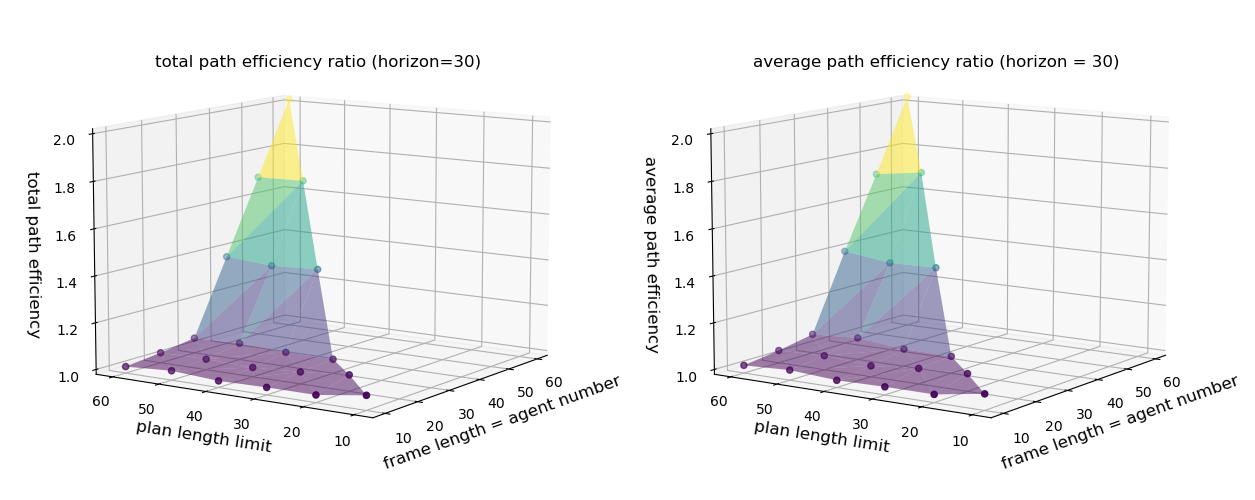
\includegraphics[width = \linewidth]{figures/horizon30_plan_length_limit_vs_performance.png}
      \caption{Experiment Group 1.1: path efficiency versus plan length limit (planning horizon = 30)}
      \label{fig:horizon=30,performance/planlengthlimit}
    \end{subfigure}
    \begin{subfigure}[t]{1.1\linewidth}
        \centering
        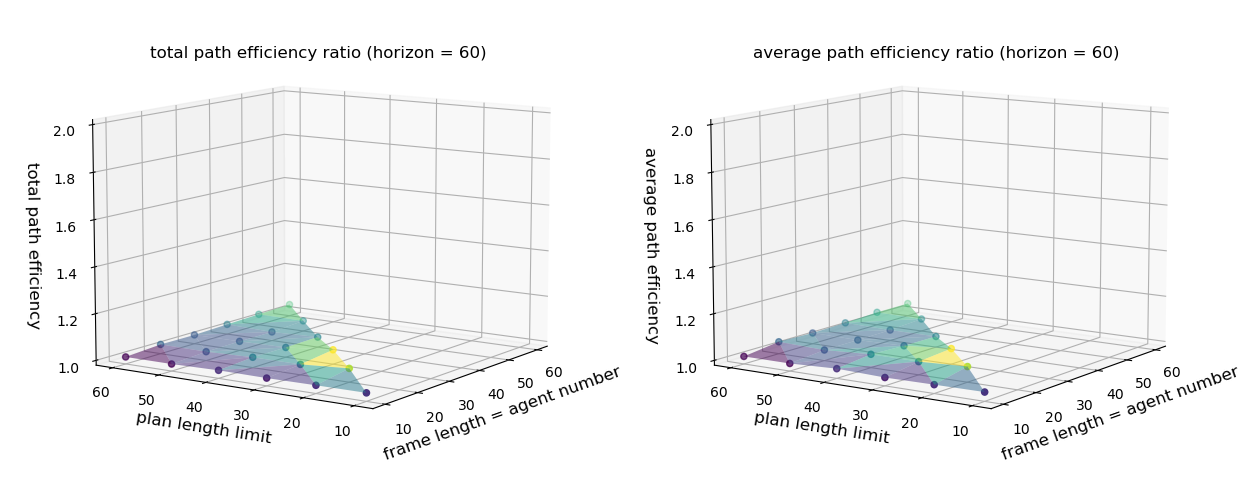
\includegraphics[width = \linewidth]{figures/horizon60_plan_length_limit_vs_performance.png}
        \caption{Experiment Group 1.2: path efficiency versus plan length limit (planning horizon = 60)}
        \label{fig:horizon=60,performance/planlengthlimit}
      \end{subfigure}
    \caption{Performance versus Planning Horizon and Plan Length Limit. The vertical axis represents performance metrics, with lower values indicating better performance.}
    \label{fig:plan_length_limit}
\end{figure}

\FloatBarrier

% Fig4.2中展示了与路径质量相关的两个metric与planning horizon及plan length limit的关系。
In Figure \ref{fig:plan_length_limit}, the relationship between two metrics (total and average path efficiency) associated with path quality and the planning horizon, as well as the plan length limit, is illustrated.
% 结果可以分为两个部分:帧长度超出planning horizon的部分和帧长度未超出planning horizon的部分。
The \textbf{results can be divided into two parts}: frame length > the planning horizon, and where the frame length < the planning horizon.

\begin{itemize}
    \item Frame Length > Planning Horizon: 
    
    % Fig 4.2.a中的斜坡部分就是这部分的结果。此部分中的frame lengt均大于planning horizon, 也就意味着在每帧的最后一部分,agent只能原地不动。
    The slope in Figure \ref{fig:horizon=30,performance/planlengthlimit} represents this part of results. Within this portion, the frame lengths are all greater than the planning horizon, indicating that agents remain stationary during the final part of each frame.

    % 在这部分中,frame length和planning horizon的关系对路径效率起主导作用。可以看出,不论是总路径效率还是平均路径效率,都几乎等于帧长度与planning horizon的比例(如在frame length = 60处为2.0)
    In this part, \textbf{the relationship between frame length and planning horizon predominantly influences path efficiency}. It's evident that both the total path efficiency and the average path efficiency nearly equal the ratio of frame length to planning horizon (as seen at frame length = 60, the ratio is near 2.0, for instance).

    \item Frame Length < Planning Horizon: 
    
    %Fig 4.2中所有剩余的平坦部分是这部分的结果。从图中可以看出,在frame length不超出planning horizon的情况下,路径效率几乎不随plan length limit变化。图中所有平坦部分的z轴(即metric)值均低于1.05.
    In Figure \ref{fig:plan_length_limit}, all the flat parts represent the results of this part. From the graph, it's evident that when the frame length does not exceed the planning horizon, path efficiency remains almost unchanged regardless of variations in the plan length limit. The z-axis values in all these flat sections of the graph are below 1.05.
    
    % 这表明:要么是plan length limit对路径效率没有显著影响,要么是地图对于实验中运行的agent来说过于开阔。
    This indicates that \textbf{either the plan length limit has negligible impact on path efficiency, or the map is too open for the agents} involved in the experiment. 
    
\end{itemize}


% 对于地图太开阔的解释:如\ref{chap:map}中所提到的一样,虽然所有的走廊都只能有1agent宽,但由于障碍物的特殊分布,当一条路径被阻挡时,agent可以简单地选择在不同的路口转弯,来在不损失路径效率的情况下避开被使用的走廊。
The explanation for the map being too open: 

As mentioned in Section \ref{chap:map}, although all the corridors have a width of only one agent's width (one grid / pixel), due to the specific distribution of obstacles, 
when a path is blocked, \textbf{an agent can simply choose to turn at different intersections to avoid collision}, 
this allows them to avoid the occupied corridors without sacrificing path efficiency.
% agent的起点终点设置\ref{chap:agent initialisation}可能加剧了这一情况,因为agent均需要跨过地图,而跨过此地图的最优路线有很多种。
The setting of agent starting and ending points, as described in \ref{chap:agent initialisation}, might contribute to this situation. 
All agents need to cross the map, and \textbf{there are many optimal routes for crossing this map}, which could exacerbate the open nature of the map.

% 总体来说,实验结果表明,对于本测试情景,plan length limit并不重要。只要frame length不超出planning horizon, 路径效率就可以保持在接近最优的水平。
Overall, these experimental results suggest that, within the context of this test scenario, 
the plan length limit is not a critical factor. 
\textbf{Provided that the frame length does not surpass the planning horizon, path efficiency may be sustained at a level closely approximating the optimum}. 
% 一旦frame length超过planning horizon,路径效率就急剧恶化,应当尽量避免这一情况发生。
\textbf{If the frame length exceed the planning horizon, there would be a dramatic deterioration in path efficiency}, and this is a situation that should be assiduously avoided.

\subsubsection{frame length and agent number}

% 这两组参数主要影响系统容量。frame length是一帧中槽的数量,agent number是同时启动agent的个数。
\textbf{These two parameters are related to the system capacity}. Frame length refers to the quantity of slots within a frame, and agent number represents the number of agents initiated simultaneously at the beginning of simmulation run.

% 帧长度较长和较短各有利弊。
\textbf{The advantages and disadvantages exist for both longer and shorter frame lengths}:
\begin{itemize}
    % 帧长度较长时,信道中有更多空间供agent使用,也就允许更多的agent加入信道。但若在加入过程中发生碰撞,根据协议,agent需要重听一整帧来重新确定分配情况来再次尝试加入,这一时长会随帧长度的增加而增加,因而帧长度并不是越长越好。
    \item Longer frame lengths:  there is more channel space available for agents, allowing a larger number of agents to join the channel. However, if collisions occur during the joining process, according to the protocol (Section \ref{chap:stdma statemachine}), agents need to re-listen to the entire frame to reconfirm the allocation and make another attempt to join. This time duration for re-listening increases with the longer frame length. Consequently, longer frame lengths do not necessarily lead to better outcomes.
    % 帧长度较短时,信道中空间不足,大量agent会停留在信道加入阶段,会导致效率的降低。此时虽然没有帧长度较长时重听一帧耗时长的弊端,但其信道容量本身就较低。
    \item Shorter frame lengths: When the frame length is shorter, there is limited channel space, which can result in a significant number of agents lingering in the channel joining phase. This can lead to reduced efficiency. Although this scenario may not suffer from the prolonged re-listening disadvantage seen with longer frame lengths, the channel capacity is low due to the shorter frame length.
\end{itemize}

% 从此处也可以看出,frame length的大小是相对于agent number的
From this perspective, it is apparent that the magnitude of the frame length is relative to the agent number.

% 为了验证帧长度的相对长短对系统性能的影响,进行如下实验:
To investigate the impact of varying frame lengths on system performance, \textbf{the following experiments are conducted}:

\begin{itemize}
    % 遍历以下的参数空间两次:planning horizon = 60, plan length limit = 60, agent number 10-60 步长为10,frame length 10-60 步长为5
    \item Group 2: The parameter space will be traversed twice with the following settings: planning horizon = 60, plan length limit = 60 (these two are independent parameters), agent number ranging from 10 to 60 with a step size of 10, and frame length ranging from 10 to 60 with a step size of 5.
    % 参数空间中的某些点由于耗时过长性能过差,予以省略
    Certain points in the parameter space (specifically, those with agent numbers significantly surpassing frame lengths) are omitted due to excessive time consumption and clearly inadequate performance.
\end{itemize}

% 实验中仍然存在与前一组实验相同的随机因素,即agent在加入信道时随机选择free slot尝试加入的这一因素。由于实验耗时比较可观(一个slot耗时1秒),仅遍历参数空间两次并取性能参数的平均值作为结果。虽然这样不能完全消除结果中的随机性,但性能随参数变化的趋势仍然表现得很明显。
Similar to the previous groups of experiments, the same random factor exists in this group as well: the randomness associated with agents randomly selecting free slots to attempt joining the channel upon entry. 
Due to the considerable time required for the experiment (with each slot taking 1 second), the parameter space is traversed only twice, and the average values of performance metrics are taken as results. 
Although this approach doesn't entirely eliminate randomness from the outcomes, the performance trends with parameter variations are still quite evident.


\begin{figure}[htbp]
    \centering
    \begin{subfigure}[t]{0.45\linewidth}
      \centering
      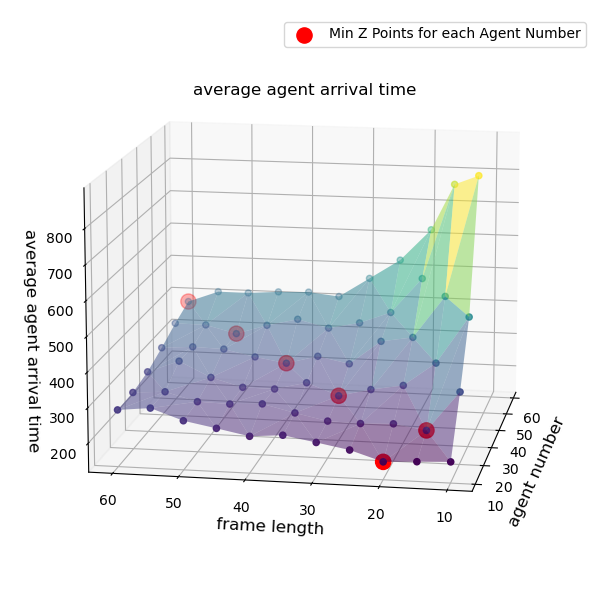
\includegraphics[width = \linewidth]{figures/avg_arrival_time.png}
      \caption{Average agent arrival time results}
      \label{fig:Performance1}
    \end{subfigure}
    \hfill
    \begin{subfigure}[t]{0.45\linewidth}
        \centering
        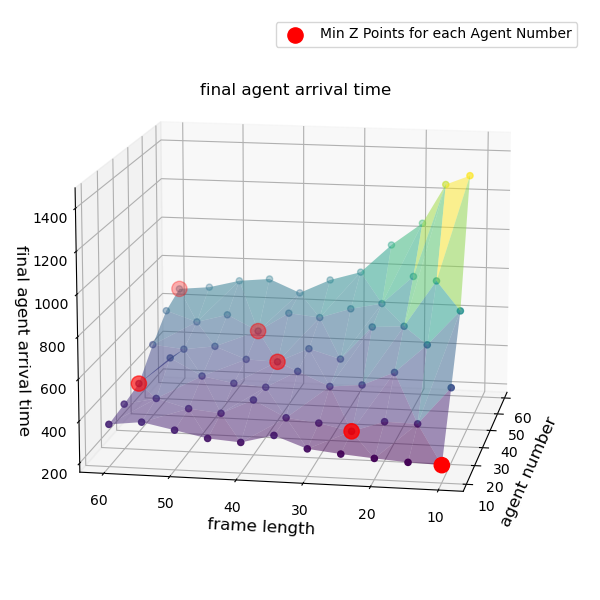
\includegraphics[width = \linewidth]{figures/final_agent_arrival_time.png}
        \caption{Final agent arrival time results}
        \label{fig:Performance2}
    \end{subfigure}
    
    \vspace{1cm}
    
    \begin{subfigure}[t]{0.45\linewidth}
        \centering
        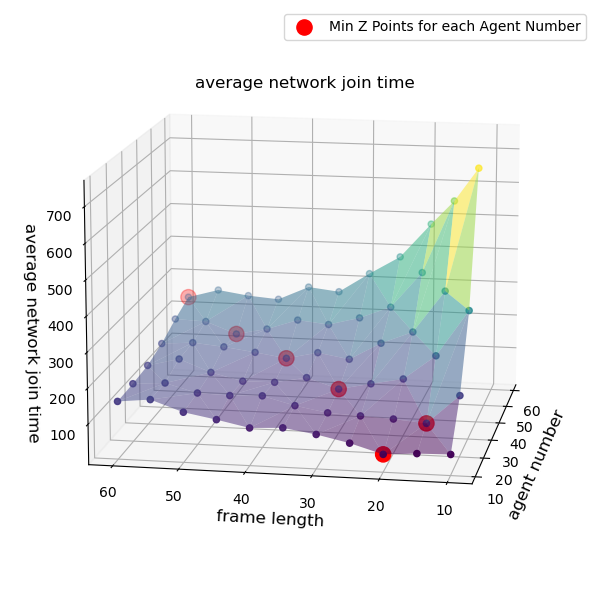
\includegraphics[width = \linewidth]{figures/avg_network_join_time.png}
        \caption{Average network join time results}
        \label{fig:Performance3}
    \end{subfigure}
    \hfill
    \begin{subfigure}[t]{0.45\linewidth}
        \centering
        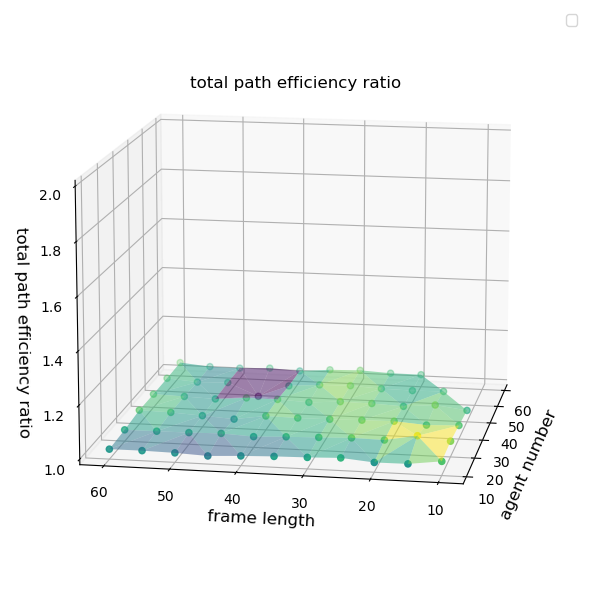
\includegraphics[width = \linewidth]{figures/total_path_effi_ratio.png}
        \caption{Total path efficiency ratio result. It is evident from this graph that path efficiency is largely unaffected.}
        \label{fig:Performance4}
    \end{subfigure}
    \caption{Experiment Group 2: Performance versus Agent number and Frame Length. The vertical axis represents performance metrics, with lower values indicating better performance.}
    \label{fig:Performance}
\end{figure}
\FloatBarrier

% 能影响最重要的参数:arrival time的因素只有两个:(1)agent加入网络的耗时。(2)agent的路径效率。
There are only two factors that can influence the most important metric, which is the arrival time. These factors are: \textbf{(1)} the duration it takes for an agent to join the network, and \textbf{(2)} the efficiency of the agent's path. 

% 而在这两个因素中,agent的路径效率在本实验场景中对arrival time的影响几乎没有,因为其本身在整个参数空间内的变化不大。
In these two factors, the \textbf{path efficiency of the agent has almost no impact on the arrival time in this experimental scenario, as its variation across the entire parameter space is minimal}.
% 从Figure \ref{fig:Performance4}可以看出,agent的路径效率始终保持在较高的水平(图中的所有点的z轴值均低于1.05,与第一组实验中的结果相同)
As can be seen from Figure \ref{fig:Performance4}, the efficiency of the agent's path is consistently high (all the points on the z-axis in the figure are below 1.05, which is in line with the results from the first group of experiments).
% Figure \ref{fig:Performance1,fig:Performance2,fig:Performance3}之间形状的相似也能证明这一点。虽然final arrival time由于更高的随机性(不像average arrival time那样由平均产生)而稍有走形,但其总体趋势仍然是一样的。
The morphological similarity among Figure \ref{fig:Performance1}, Figure \ref{fig:Performance2}, and Figure \ref{fig:Performance3} lends further credence to this observation, as the shape of the arrival time closely mirrors that of the time consumed by agents when joining the network.
Although the final arrival time may deviate slightly due to higher randomness (as opposed to the average arrival time which is generated by averaging), the overall trend remains consistent.


% 因此,本实验场景中的性能参数主要由agent加入网络的耗时决定。性能在参数空间中的变化可以从这一方面来解释。
\textbf{Consequently, the performance parameters in this scenario are primarily determined by the time it takes for an agent to join the network.} The variation in performance across the parameter space can be explained from this perspective.


% 从图中可以看出,对于每个agent number,性能最优的点集中在agent number与frame length值接近或相等的地方。这一现象可以从以下两方面解释:
As can be seen from Figure \ref{fig:Performance1}, \ref{fig:Performance2}, \ref{fig:Performance3}, for each agent number, 
the points of \textbf{optimal performance tend to concentrate where the agent number and frame length values are close or equal}. 
% 以agent number = frame length的线为界,可以将结果分为两部分讨论:
Using the line where agent number = frame length as a reference, the results can be divided into two parts for discussion:

\begin{itemize}
    \item Agent Number < Frame Length:
    
    This part corresponds to the upper-right part of each figure in  Fig \ref{fig:Performance}. 
    When the agent number increases relative to the frame length, there is a significant negative impact on performance.
    
    % 这是因为此时信道容量过小,一部分agent必须待机,直到信道中有可用空间出现,才能开始运行。
    This is because, in this part, the channel capacity is relatively limited, and a portion of agents must remain idle until available channel space emerges, allowing them to start their operations (entering the map).
    
    \item Agent Number > Frame Length
    
    This part corresponds to the bottom-left part of each figure in Fig \ref{fig:Performance}. 
    As the frame length increases relative to the agent number, the performance gradually declines.
   

    % 此时,channel的容量允许全部agent在网络中运行,但是根据协议,若多个agent在尝试加入网络时发生碰撞(碰巧尝试占用同一个空闲槽位),则在下一次尝试之前必须听完完整的一帧。这一机制使得过长的frame length对agent join time有负面影响。
    In this part, the channel has enough capacity for all the agents to operate in the network at same time. 
    However, according to the protocol (Section \ref{chap:stdma statemachine}), if multiple agents collides in the channel (accidentally trying to occupy the same free slot when entering), they must wait and listen through an entire frame before attempting again. 
    This mechanism means that an excessively long frame length has a negative impact on the agent join time, as the extended frame length prolongs the time needed for each retry.

\end{itemize}


% 这就可以理解为什么对于每个agent number来说,性能最优的点大多是frame length = agent number或稍高于 agent number。因为此时信道中有足够的位置,不会出现只能待机的agent,同时帧长度又没有过长,加入网络中重试的过程不会耗时过长。
This explains why, for each agent number, \textbf{the points with the optimal performance are mostly when the frame length equals the agent number or slightly higher than the agent number}. In these cases, there is enough room in the channel to avoid having agents solely in idle mode, while the frame length is also not excessively long, preventing a prolonged process of retrying to join the network.


\subsubsection{Channel Utilization}

% 对于使用stdma分享信道的agent来说,信道并不总是满的。实际上,信道的一部分总是被许多未能获得槽的agent争抢,它们在其中相互碰撞。
For agents using STDMA to share channels, \textbf{the channels aren't always full}. In fact, \textbf{a portion of the channel is always contended for by numerous agents that haven't secured a slot}, leading to mutual collisions among them.
% 我们通过观察不同agent数量下信道的使用率来分析此问题。
This concern is investigated by examining the channel usage rate as a function of varying numbers of agents, while keeping the frame lengths constant.

% 从Group2的两次重复实验中取一次结果绘制成图(Fig \ref{fig:channelpercent})。虽然这样不能去除实验中的随机性,但整体趋势不受这种随机性影响。
One set of results from two repeated experiments in Group 2 is illustrated in Figure \ref{fig:channelpercent}. While this method does not remove the element of randomness present in the experiment, the overall trend observed in the results remains unaffected by such randomness.

\begin{figure}[htbp]
    \centering
    % Row 1
    \begin{subfigure}[t]{0.45\linewidth}
        \centering
        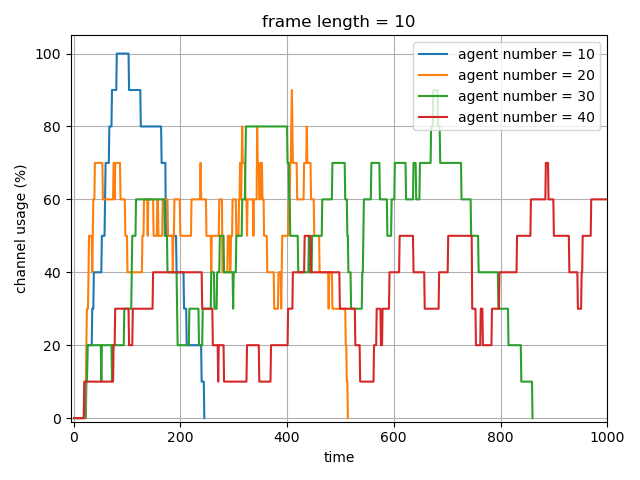
\includegraphics[width=\linewidth]{figures/channel_usage_frame10.png}
        \caption{frame length = 10}
        \label{fig:framepercent1}
    \end{subfigure}
    \hfill
    \begin{subfigure}[t]{0.45\linewidth}
        \centering
        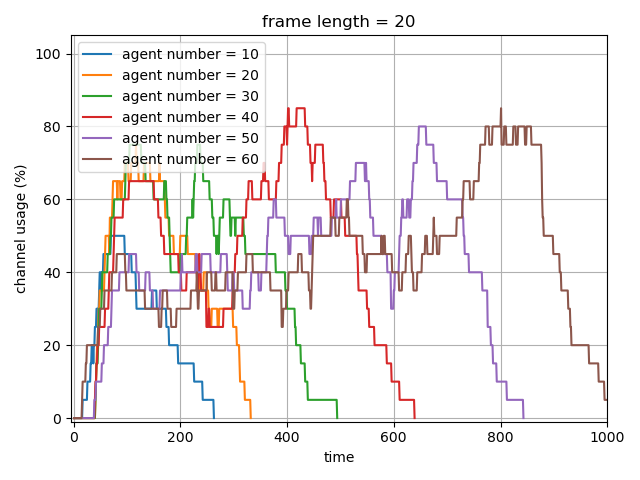
\includegraphics[width=\linewidth]{figures/channel_usage_frame20.png}
        \caption{frame length = 20}
        \label{fig:framepercent2}
    \end{subfigure}
    
    \vspace{1cm}
    
    % Row 2
    \begin{subfigure}[t]{0.45\linewidth}
        \centering
        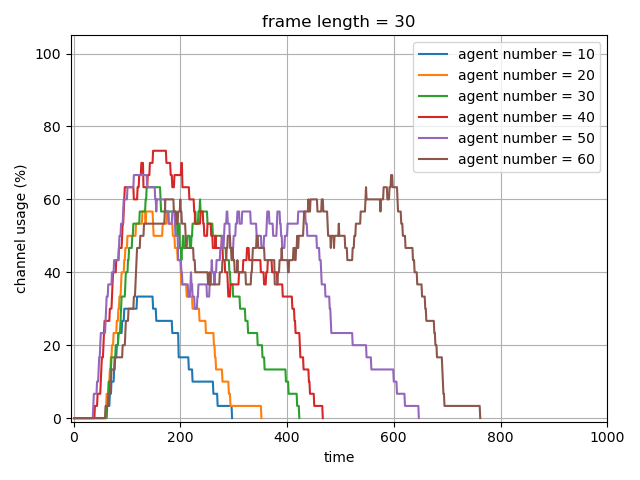
\includegraphics[width=\linewidth]{figures/channel_usage_frame30.png}
        \caption{frame length = 30}
        \label{fig:framepercent3}
    \end{subfigure}
    \hfill
    \begin{subfigure}[t]{0.45\linewidth}
        \centering
        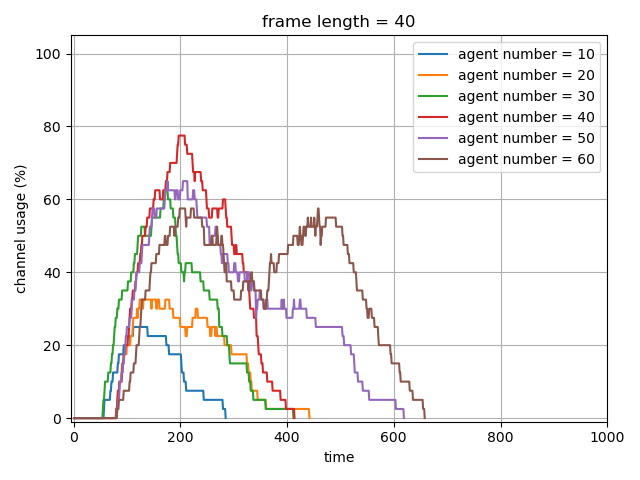
\includegraphics[width=\linewidth]{figures/channel_usage_frame40.png}
        \caption{frame length = 40}
        \label{fig:framepercent4}
    \end{subfigure}
    
    \vspace{1cm}
    
    % Row 3
    \begin{subfigure}[t]{0.45\linewidth}
        \centering
        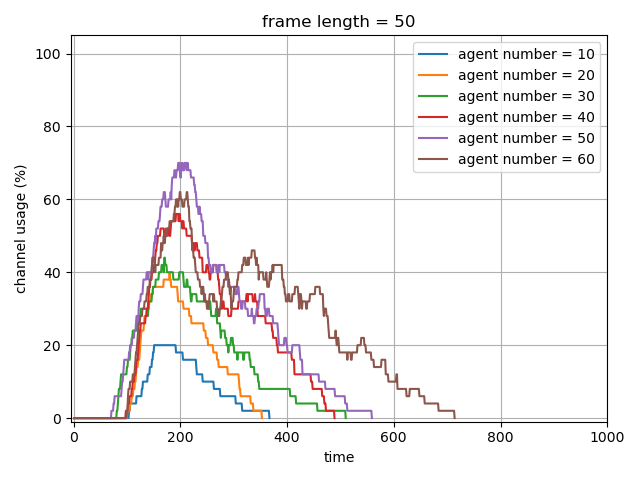
\includegraphics[width=\linewidth]{figures/channel_usage_frame50.png}
        \caption{frame length = 50}
        \label{fig:framepercent5}
    \end{subfigure}
    \hfill
    \begin{subfigure}[t]{0.45\linewidth}
        \centering
        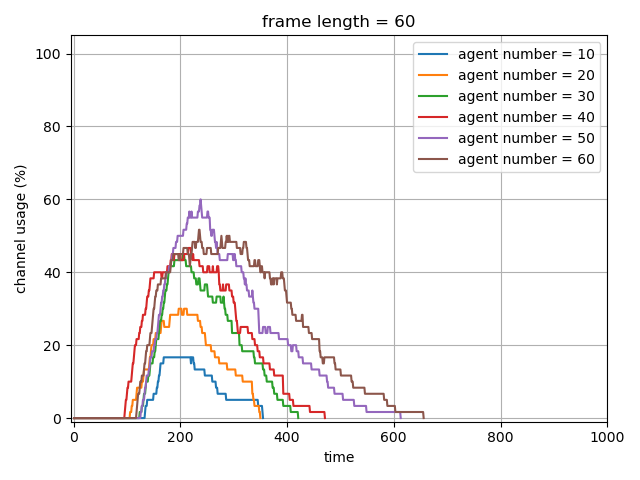
\includegraphics[width=\linewidth]{figures/channel_usage_frame60.png}
        \caption{frame length = 60}
        \label{fig:framepercent6}
    \end{subfigure}
    
    \caption{Graph illustrating the relationship between the percentage of channel usage and time, for varying numbers of agents.}
    \label{fig:channelpercent}
\end{figure}


% 2. 信道使用率最高在80%左右(除去Figure \ref{fig:framepercent1}中10 agent, frame length = 10这种小规模的情况)。
% 3. agent数量越是与frame length接近,对信道的使用率越高。可以从两方面看出这一点:
%    - 最先达到峰值的是与frame length较接近的agent number的曲线
%    - 若agent number大大超过frame length,则此组对于信道的使用率会逐渐上升,因为完成任务的agent逐渐下降,系统中的活动agent数量减少,使其逐渐接近agent number = frame length。
% 从Figure \ref{fig:channelpercent}中,可以看出以下几条:
\textbf{From Figure \ref{fig:channelpercent}, we can deduce the following points}:
\begin{enumerate}
    \item 
    The highest channel usage rate is around 80\%, excluding small-scale scenarios like 10 agents with a frame length of 10 as seen in Figure \ref{fig:framepercent1}.
    \item 
    The channel usage rate is higher when the number of agents is closer to the frame length. This can be observed in two ways:
    \begin{itemize}
        \item 
        The first curves in each figure to reach their peak are those where the number of agents is closer to the frame length.
        \item
        If the number of agents far exceeds the frame length (e.g., Fig \ref{fig:framepercent2}, \ref{fig:framepercent3}), the channel usage rate for this group gradually increases. This is because the number of agents completed tasks rises, reducing the number of active agents in the system, making it gradually approach the scenario where the number of agents equals the frame length.
    \end{itemize}
\end{enumerate}


\subsubsection{Portion of Agents in Channel}

% 在本算法的条件下,只有在信道中的agent才可以发布计划并在地图中运动,因此在信道中的agent的比例值得关注。
% 我们通过观察不同frame length下agent在信道中的比例来观察此问题。
In the implemented algorithm, \textbf{only agents present in the channel can publish plans and move within the map. Hence, the proportion of agents in the channel is worthwhile to take a look}.
We delve into this matter by analysing the proportion of agents in the channel across different frame lengths.

% 仍然和Channel Ultilization使用同一组数据。事实上,信道中agent的比例可以视为channel ultilization的另一个观察角度
The same dataset used for Channel Utilization observation is still employed here. In fact, the proportion of agents in the channel can be viewed as another perspective on Channel Utilization.

\begin{figure}[htbp]
    \centering
    % Row 1
    \begin{subfigure}[t]{0.45\linewidth}
        \centering
        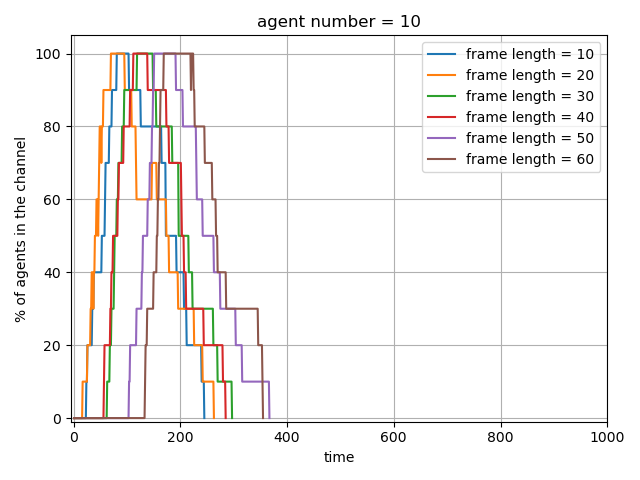
\includegraphics[width=\linewidth]{figures/channel_usage_agent10.png}
        \caption{10 agents}
        \label{fig:agentpercent1}
    \end{subfigure}
    \hfill
    \begin{subfigure}[t]{0.45\linewidth}
        \centering
        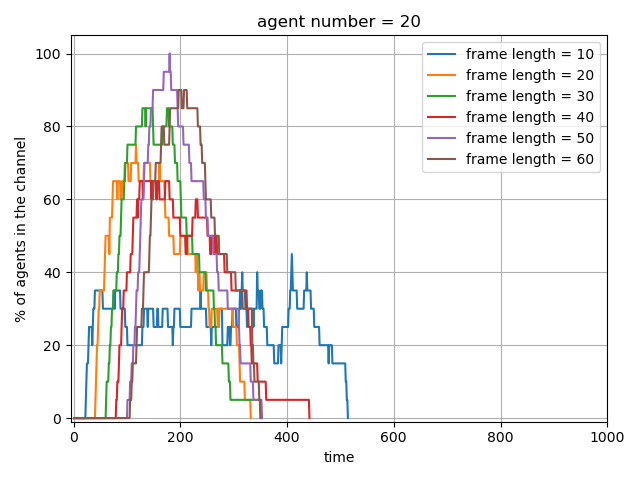
\includegraphics[width=\linewidth]{figures/channel_usage_agent20.png}
        \caption{20 agents}
        \label{fig:agentpercent2}
    \end{subfigure}
    
    \vspace{1cm}
    
    % Row 2
    \begin{subfigure}[t]{0.45\linewidth}
        \centering
        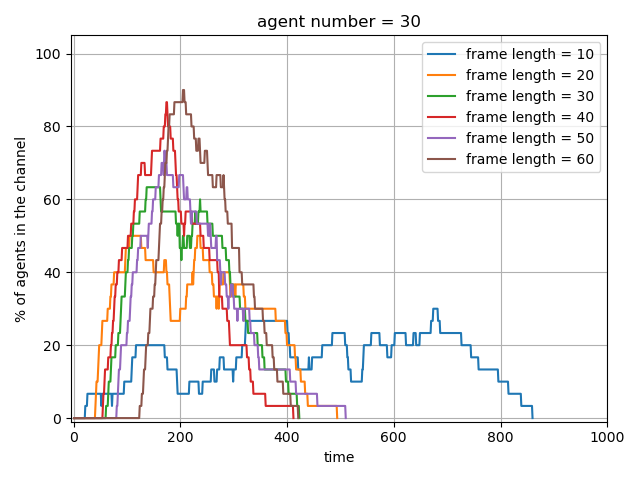
\includegraphics[width=\linewidth]{figures/channel_usage_agent30.png}
        \caption{30 agents}
        \label{fig:agentpercent3}
    \end{subfigure}
    \hfill
    \begin{subfigure}[t]{0.45\linewidth}
        \centering
        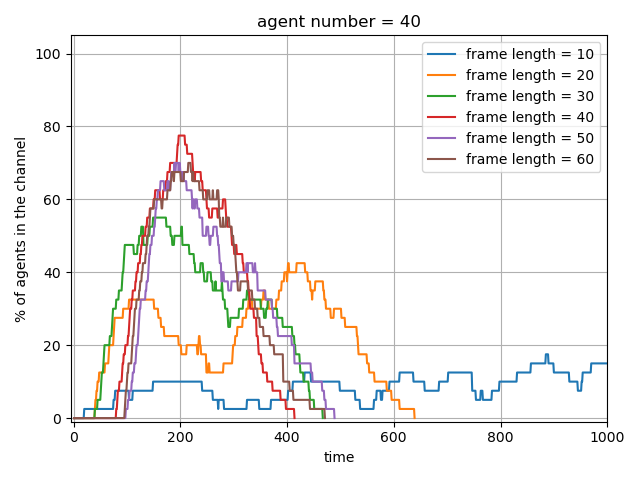
\includegraphics[width=\linewidth]{figures/channel_usage_agent40.png}
        \caption{40 agents}
        \label{fig:agentpercent4}
    \end{subfigure}
    
    \vspace{1cm}
    
    % Row 3
    \begin{subfigure}[t]{0.45\linewidth}
        \centering
        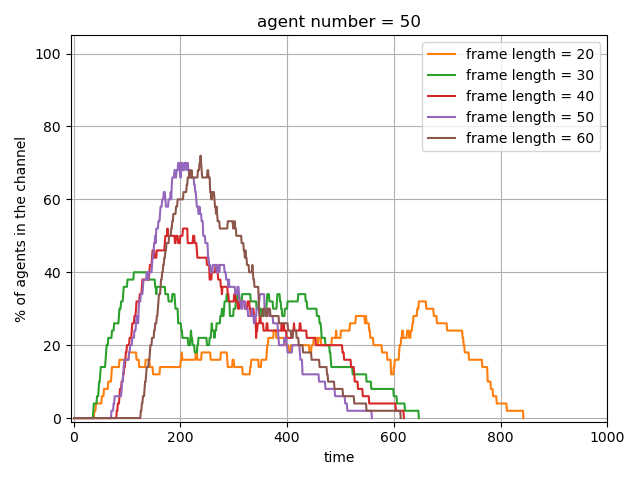
\includegraphics[width=\linewidth]{figures/channel_usage_agent50.png}
        \caption{50 agents}
        \label{fig:agentpercent5}
    \end{subfigure}
    \hfill
    \begin{subfigure}[t]{0.45\linewidth}
        \centering
        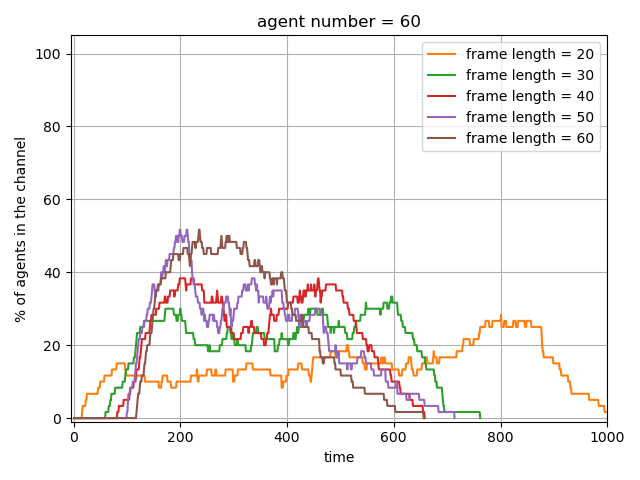
\includegraphics[width=\linewidth]{figures/channel_usage_agent60.png}
        \caption{60 agents}
        \label{fig:agentpercent6}
    \end{subfigure}
    
    \caption{Graph depicting the correlation between the percentage of agents in the channel and time, across varying agent quantities and frame lengths.}
    \label{fig:agentpercent}
\end{figure}

% 从Figure \ref{fig:agentpercent}中,可以得到以下信息:
\textbf{From Figure \ref{fig:agentpercent}, we can deduce the following points:}
\begin{enumerate}
    \item 
    % 1. 当frame length高于agent number时,可以允许更多的agent同时存在于信道中,但帧越长,agent加入信道的耗时就越长,在图中表现为达到峰值较慢,如 Fig \ref{fig:ageentpercent1}中,虽然所有frame length都可以使全部agent进入channel, 但是frame length越长,达到峰值越慢。
    Frame Length > Agent Number: More agents can enter the channel. However, \textbf{the longer the frame, the more time it takes} to reach the peak percentage, manifesting as a slower rise to peak values in the graph (e.g., Fig \ref{fig:agentpercent1}).
    \item 
    % 2. 当agent number 超过frame length时,在信道中的agent数量显著减少,不只是因为帧中没有足够的空间,也因为有太多的agent争抢空闲槽位。随着agent逐渐减少(陆续完成任务),信道中的agent数量反而提升(e.g., Fig \ref{fig:agentpercent3} 中frame length = 20的曲线)
    Frame Length < Agent Number: The portion of agents in the channel drops notably. This decrease isn't solely due to the lack of enough space in the frame but also because \textbf{too many agents are contending for the available slots}. As agents progressively decrease (as they complete their tasks over time), the number of agents in the channel increases (e.g., the curve for frame length = 20 in Fig \ref{fig:agentpercent3}, \ref{fig:agentpercent4}, \ref{fig:agentpercent5}, \ref{fig:agentpercent6}).
    \item 
    % 3. 当frame length在agent number左右的时候,在信道中的agent的百分比的峰值大约保持在60%左右,这一值随着frame length增加而上升,随frame length减少而减少。
    Frame Length $\approx$ Agent Number: The peak percentage of agents in the channel stabilizes at around 60\%. This value increases with a rise in frame length and decreases as the frame length diminishes.
\end{enumerate}    
\FloatBarrier

\subsection{Back-off Behaviours Arising from Optimal 3D Path Planning}

% 由于agent所寻找的最优路径是在3维空间中的(2D平面坐标+时间),agent会做出一些从2D角度看来是退避的动作。如下图所示。
Because agents are searching for optimal paths within a 3D space—consisting of 2D planar coordinates and time—it is observed that agents may take actions that appear as retreats when viewed from a 2D perspective. Some typical examples are illustrated in the figure below:

\begin{figure}[htbp]
    \begin{subfigure}[t]{0.45\linewidth}
        \centering
        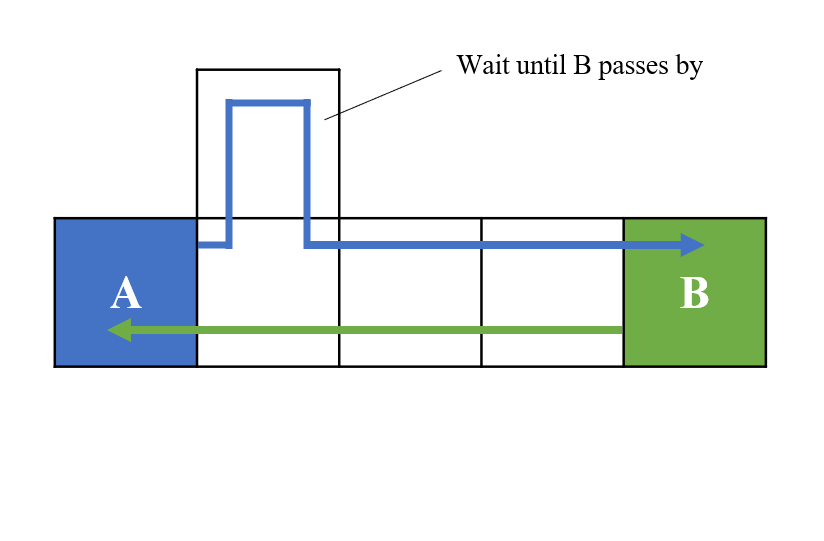
\includegraphics[width=\linewidth]{figures/Retreat1.png}
        \caption{Illustration of a narrow corridor with adjacent extra area. A utilizes the extra area to wait for B to pass.} % 带有一块额外区域的窄走廊。A会在额外区域中等待,直到B通过。
        \label{fig:retreat1}
    \end{subfigure}
    \hfill
    \begin{subfigure}[t]{0.45\linewidth}
        \centering
        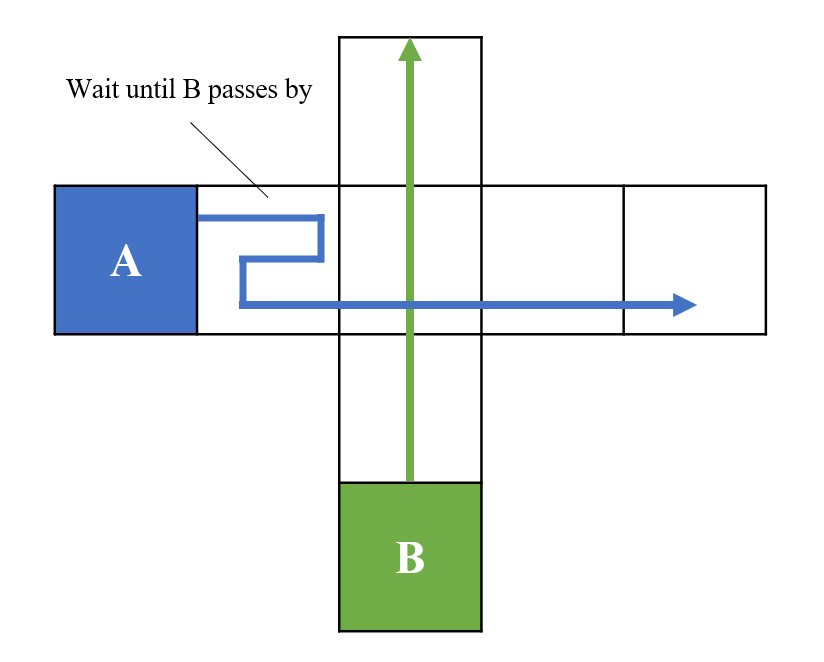
\includegraphics[width=\linewidth]{figures/Retreat2.png}
        \caption{Illustration of an intersection meeting. A waits for B to cross before proceeding.}% 十字路口。A会等待B通过十字路口交叉点,然后再前进。
        \label{fig:retreat2}
    \end{subfigure}
    \caption{Illustration of typical back-off scenarios, wherein agent A formulates plans based on the plan received from agent B.}% 一些典型的退让场景。图示为A在接收到B的计划后做出的对应计划。
    \label{fig:retreat}
\end{figure}
\FloatBarrier

% 这种退让行为对于在二维空间中仅专注于寻找agent自身最优路径的算法来说是不寻常的。一个原因是进行计划的agent无条件对其他agent进行避让(生成的计划需遵循无碰撞约束),另一原因是本文中agent实际上是在由位置和时间构成的三维空间中进行无碰撞路径规划。
Such back-off behavior is unusual for algorithms that are solely focused on finding the agent's own optimal path within a two-dimensional space.
\textbf{One reason for this is that the planning agent unconditionally avoids other agents} (as the generated plans must adhere to a collision-free constraint). 
Another reason is that in the implemented algorithm, \textbf{agents are conducting collision-free path planning within a 3D space composed of both 2D position and time. This expanded planning dimension grants agents a more nuanced and comprehensive decision-making perspective}.

% 在某些场景中的行为
\subsection{Deadlock Situation}

A deadlock situation arises only under exceptionally strict conditions.

\subsubsection{Condition}
% 满足下述情况时,agent之间发生死锁:
When the following conditions are simultaneously met, a deadlock between agents occurs:

\begin{enumerate}
    \item Two agents are positioned within a sufficiently long corridor that's only one agent wide, each agent starts from different sides of the corridor and needs to reach the opposite end of this corridor.
    % agent发布计划的长度必须大于等于frame length
    \item The length of plans published by agents = frame length, i.e., planning horizon $\geq$ frame length and plan length limit = frame length.
    % 当一方开始计划时,另一方的计划应当执行了半frame length长度,而剩余半frame length的计划中包含正在计划的一方的当前位置或当前位置的相邻点,且另一方的计划为向自己的目的地前进。
    \item When one agent begins its planning, the other agent's plan should already be halfway executed, 
    with only half a frame length remaining. 
    \begin{itemize}
        \item This yet-to-be-executed half of the plan should contain the current or adjacent position of the planning agent, which means this yet-to-be-executed part interferes the new plan of the planning agent. 
        \item The content of this half frame length plan should be solely directed towards its goal (advancing).
    \end{itemize}
\end{enumerate}
% 解释:为什么此种情况会发生死锁
\subsubsection{Explanation}

% 由于stdma的特性,两个agent的计划是轮流制订的,因为它们的计划时间窗就是它们的slot。同时,agent每次发布的计划长度是全局一致的。
Because the characteristic of STDMA, the two agents make plan in turns, as their planning time window is their slot in the repeating frame.
Additionally, agents publish plans of the same length throughout the entire system (see Section \ref{chap:model prediction}).

% 在这一情况下,agent的计划可以分为两部分:
In this scenario, an agent's plan could be divided into two parts:
\begin{itemize}
    % 1. 后退:受到无碰撞约束的影响,当对方在计划中前进时必须后退
    \item Retreating: Due to collision-free constraints, when the other agent is moving forward in its plan, the agent must retreat to avoid collision.
    % 2. 前进:己方计划时,在planning horizon的后面,对方的计划已用尽,这时可以不受对方计划的影响而前进。
    \item Advancing: When planning and in the later part of the planning horizon, the other agent's plan has exhausted (and at this point, the planning agent doesn't assume that another agent will idle after its plan ends, because a sufficient plan has already been published for it to use until its next planning window.). The planning agent could fill the rest part of its new plan with actions of proceeding toward its goal.
\end{itemize}

% 当前进和后退两部分长度相等时,就会陷入一种动态的死锁:双方各自花一半的计划用于前进,另一半用于后退。
When the lengths of the advancing and retreating segments are equal, a dynamic deadlock scenario emerges: 
both agent spend half of their plans for advancing and the other half for retreating.



\begin{figure}[htbp]
    \centering
    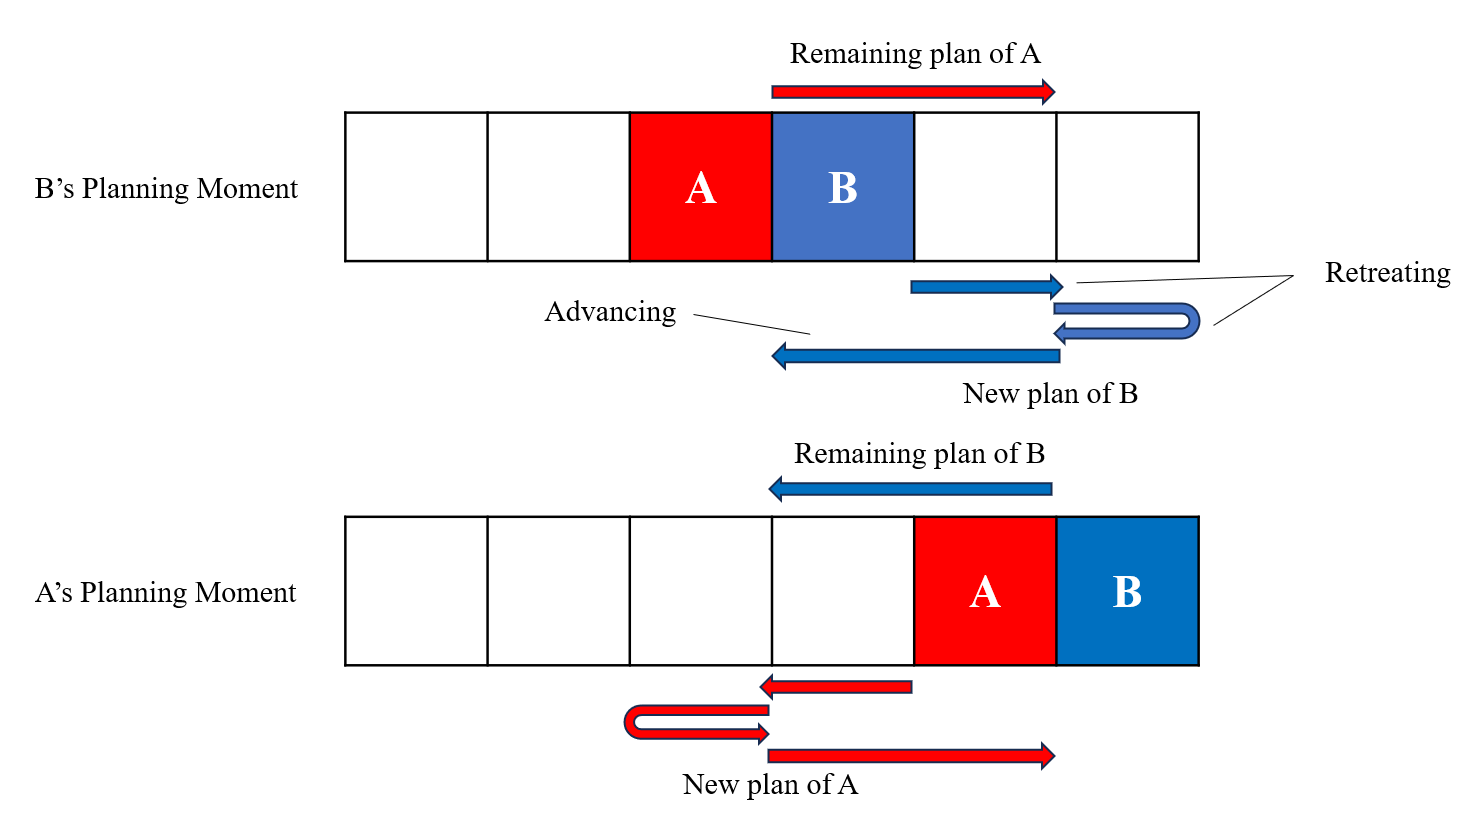
\includegraphics[width = \linewidth]{figures/deaclock_1.png}
    \caption{Example of a deadlock situation (frame length = 4, agent publishes plan with a length of 4).}% 死锁情况示例。(frame length = 4)
    \label{fig:deadlock}
\end{figure}
\FloatBarrier

\subsubsection{Solution}

% 由于此死锁情景的苛刻要求,只要打破条件1,2,3中的任意一个即可。
Due to the stringent requirements of this deadlock scenario, breaking any one of the three conditions will suffice.

For example:
\begin{itemize}
    \item Use odd-numbered frame length: This breaks the tie between advancing and retreating, because these two parts cannot be of equal length.
    \item Avoid using long narrow corridors: Add additional area to the corridor, don't force agents to push each other.
    \item Allow agents to publish longer plans:
     % 因为一方提前预定了很长空间用于前进,另一方必须在计划中对应的部分后退,这使得前进-后退的循环非常不均衡,从而可以快速离开走廊区域。
     If one agent requests an extensive span of space in their plan for advancing, the other agent will be compelled to retreat in the corresponding part of its plan. This results in a highly imbalanced advance-retreat cycle, facilitating a swift exit from the corridor area.
\end{itemize}

% 此情景在生成量化结果时未出现,因为测试地图中的障碍物相对于测试中使用的planning horizon足够小,且此情景本身出现条件比较苛刻。
This situation didn't show up in the quantitative result generating. This is mostly because the obstacles on our test map were relatively small compared to the planning horizon applied, so one agent could book all space in the corridor for advancing in one plan. Also, the conditions for this situation is quite strict.

\subsection{Failure Situation}

In the deadlock scenario, if there is a third agent, it could result in a failure: agent in the middle cannot find any possible plan.

\subsubsection{Condition}

\begin{enumerate}
    \item Three agents are positioned within a sufficiently long corridor that's only one agent wide.
    \item All agents are trying to get from one side of the corridor to the other, and one agent's starting and ending points are the complete opposite of the other two agents' starting and ending points.
\end{enumerate}

\begin{figure}[htbp]
    \centering
    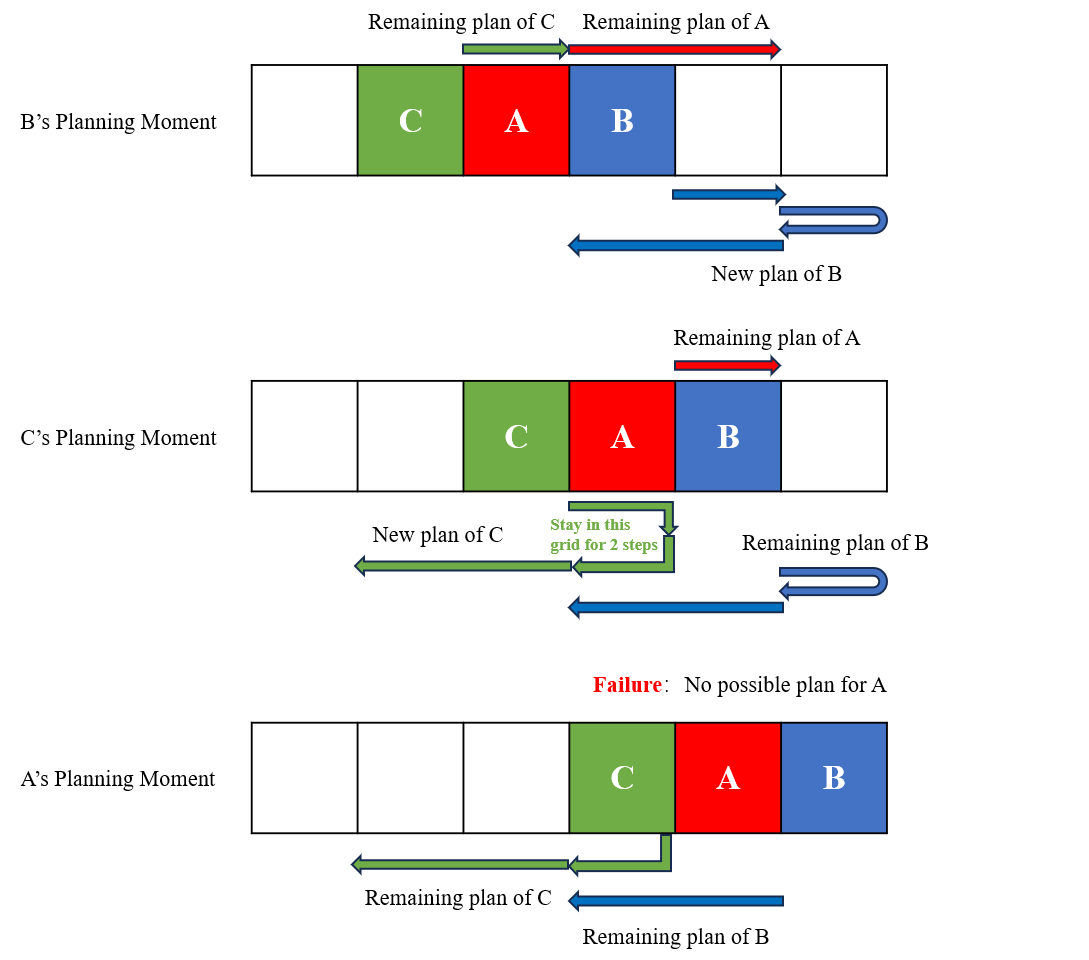
\includegraphics[width = \linewidth]{figures/Failure.png}
    \label{fig:failure}
    \caption{Example of failure. Due to the squeeze of agent C, agent A cannot find any possible plan (frame length = 4, agent publishes plan with a length of 4).}
\end{figure}

\subsubsection{Explanation}

% 此情况发生的主要原因是位于同一侧的两个agent之间的冲突。
The primary reason this situation arises is due to the conflict between the two agents on the same side of the corridor.
% 由于agent顺序计划,总会发生如下情景:
Since agents plan sequentially, the following scenario will always occur among the two agents on the same side:
\begin{itemize}
    \item 
    % 位于最外侧的agent在计划时,内侧的agent计划用尽,于是外侧agent认为可以继续前进,从而前进到与对侧agent相邻的位置
    When the outermost agent (C in Fig \ref{fig:deadlock}) is planning, the inner agent's plan exhaust within the planning horizon, leading the outermost agent to believe it can keep moving forward, subsequently advancing to a position adjacent to the agent on the opposite side.
    \item 
    % 当内侧的agent(也就是三个agent中位于中间的agent)进行计划时,由于外侧agent的挤压,无足够空间供其使用。
    When the inner agent (A in Fig \ref{fig:deadlock}, the one in the middle of the three agents) plans next, there isn't enough space for it due to the squeeze from the outer agent.
\end{itemize}

\subsubsection{Solution}

\begin{itemize}
    \item
    When the plan length that an agent can publish is sufficiently long relative to the length of the corridor, allowing an agent to reserve most of the space in the corridor in advance for its progression can prevent this situation (as seen in previous experiments where this situation didn't arise).
    \item 
    Modify the consensus among agents. Currently, an agent only assumes other agents will remain stationary after their plans run out if the published plan length of the other agents is less than one frame (see Section \ref{chap:model prediction}). If, during planning, agents always assume that other agents will stay in place once their plans are exhausted, this situation can be avoided. However, it might lead to potential decreases in path efficiency.
    \item 
    Avoid using overly long narrow corridors.
\end{itemize}


\subsection{Local Optimal Trap}

% 当障碍物足够大,agent在单个planning horizon 无法越过时,则会陷入一个局部最优陷阱中。
When an obstacle is sufficiently large such that an agent cannot surpass it within the planning horizon, the agent can become ensnared in a local optimal trap.
% agent会在障碍物内侧离终点最近的位置上保持静止,因为无法在单个planning horizon中到达比此点更接近终点的点。
The agent will remain stationary at the position inside the obstacle that is closest to the goal, as it cannot reach a position closer to the goal within a single planning horizon.

% 这是因为每次agent计划时都仅遍历一定horizon内的可能计划,然后选择这些计划中最后位置离终点最近的。
This occurs because each time the agent plans, it only explores potential plans within a certain horizon and then selects the one where the final position is closest to the goal.
% 如果horizon足够长,则可以克服此问题
If the planning horizon is long enough, this problem could be overcome.

\begin{figure}[htbp]
    \centering
    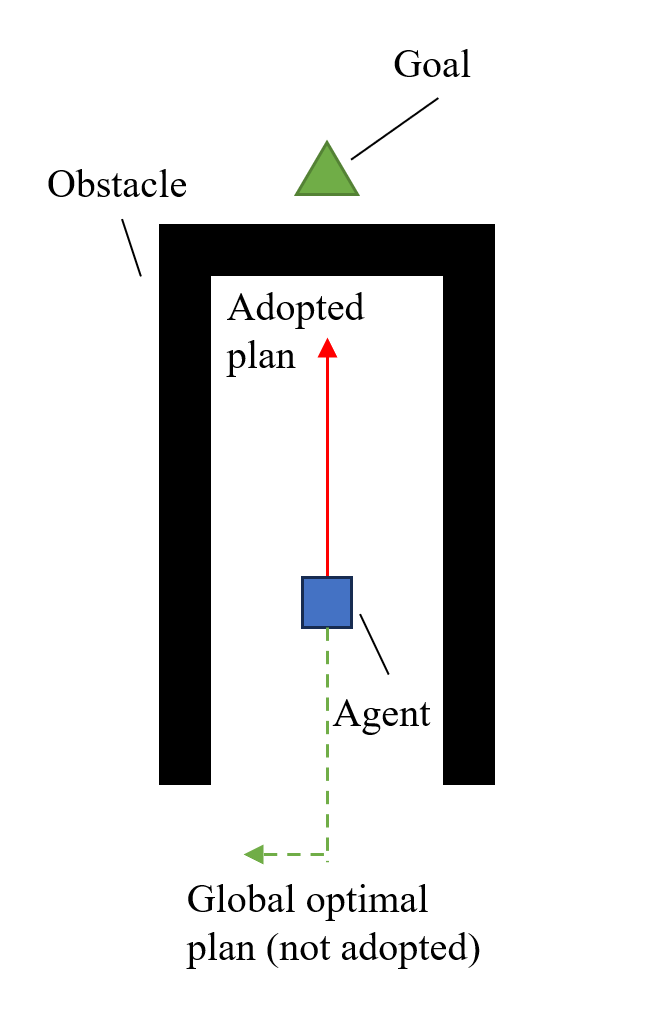
\includegraphics[width = 0.34\linewidth]{figures/Local Optimal Trap.png}
    \label{fig:LocalOptimalTrap}
    \caption{An agent trapped in a local optimum due to a short planning horizon, preventing its arrival.}% agent由于planning horizon较短,陷入局部极值陷阱并无法离开
\end{figure}
\FloatBarrier

This situation didn't show up in the quantitative result generating. This is mostly because the obstacles on our test map were relatively small compared to the planning horizon applied.




\chapter{Discussion and Conclusion}
% please replace this text with your own
The conclusion needs to provide
\begin{itemize}
    \item A short summary (What has been done and what are the main results)
    \item Limitations of your work, where applicable. 
    \item Discussion of your work in the bigger picture (How does this contribute to the research field?)
    \item Future work (What could be next steps in this work?).  Remember to keep future work realistic.  A good approach is to discuss what the next progression of this project would be, and to justify why this would be interesting.  
\end{itemize}

You will find it easier to write your conclusion if you copy-and-paste your \emph{Aims, Objectives}, and any research questions or hypotheses you stated.  You can then discuss each of these explicitly in turn, and how you were able to answer them or complete them successfully.  When things have not gone as well as you would have hoped, demonstrate your critical thinking and reasoning to analyse the short-comings of your project - to demonstrate that you understand the underlying causes and that you could conduct good futurework from this learning experience.  
\vfill



%%%%%%%%%%%%%%%%%%
\appendix
\input{appendix}  % uncomment  these two lines of code if you have don't have an appendix!

\printbibliography[ title= References]\addcontentsline{toc}{chapter}{References}


\end{document}
